% Created by tikzDevice version 0.11 on 2018-05-23 13:32:33
% !TEX encoding = UTF-8 Unicode
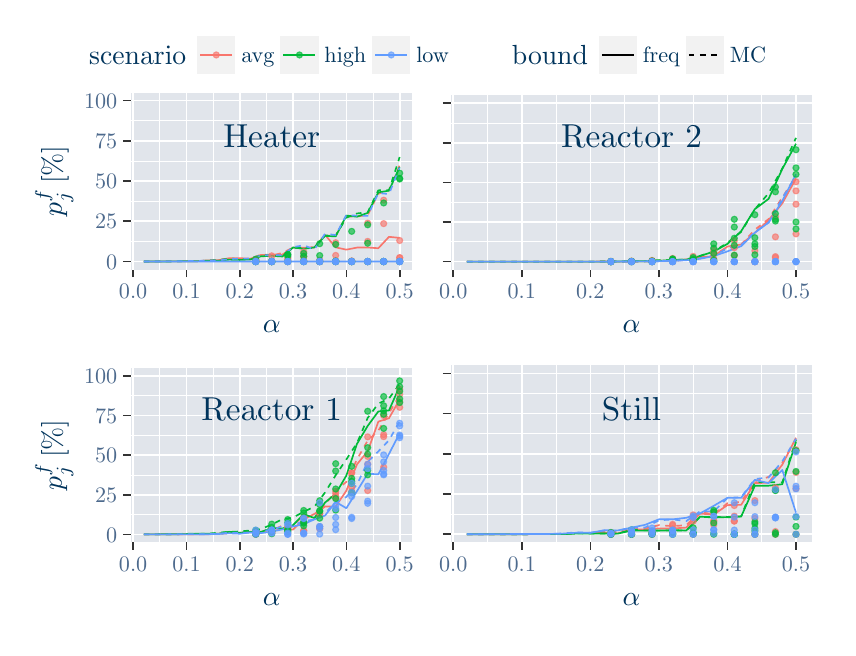
\begin{tikzpicture}[x=1pt,y=1pt]
\definecolor{fillColor}{RGB}{255,255,255}
\path[use as bounding box,fill=fillColor,fill opacity=0.00] (0,0) rectangle (289.08,216.81);
\begin{scope}
\path[clip] (  0.00, 98.55) rectangle (144.54,197.10);
\definecolor{drawColor}{RGB}{255,255,255}
\definecolor{fillColor}{RGB}{255,255,255}

\path[draw=drawColor,line width= 0.6pt,line join=round,line cap=round,fill=fillColor] (  0.00, 98.55) rectangle (144.54,197.10);
\end{scope}
\begin{scope}
\path[clip] ( 37.33,129.40) rectangle (139.04,193.34);
\definecolor{fillColor}{RGB}{225,229,235}

\path[fill=fillColor] ( 37.33,129.40) rectangle (139.04,193.34);
\definecolor{drawColor}{RGB}{255,255,255}

\path[draw=drawColor,line width= 0.3pt,line join=round] ( 37.33,139.57) --
	(139.04,139.57);

\path[draw=drawColor,line width= 0.3pt,line join=round] ( 37.33,154.10) --
	(139.04,154.10);

\path[draw=drawColor,line width= 0.3pt,line join=round] ( 37.33,168.63) --
	(139.04,168.63);

\path[draw=drawColor,line width= 0.3pt,line join=round] ( 37.33,183.16) --
	(139.04,183.16);

\path[draw=drawColor,line width= 0.3pt,line join=round] ( 47.74,129.40) --
	( 47.74,193.34);

\path[draw=drawColor,line width= 0.3pt,line join=round] ( 67.00,129.40) --
	( 67.00,193.34);

\path[draw=drawColor,line width= 0.3pt,line join=round] ( 86.26,129.40) --
	( 86.26,193.34);

\path[draw=drawColor,line width= 0.3pt,line join=round] (105.52,129.40) --
	(105.52,193.34);

\path[draw=drawColor,line width= 0.3pt,line join=round] (124.79,129.40) --
	(124.79,193.34);

\path[draw=drawColor,line width= 0.6pt,line join=round] ( 37.33,132.30) --
	(139.04,132.30);

\path[draw=drawColor,line width= 0.6pt,line join=round] ( 37.33,146.83) --
	(139.04,146.83);

\path[draw=drawColor,line width= 0.6pt,line join=round] ( 37.33,161.37) --
	(139.04,161.37);

\path[draw=drawColor,line width= 0.6pt,line join=round] ( 37.33,175.90) --
	(139.04,175.90);

\path[draw=drawColor,line width= 0.6pt,line join=round] ( 37.33,190.43) --
	(139.04,190.43);

\path[draw=drawColor,line width= 0.6pt,line join=round] ( 38.10,129.40) --
	( 38.10,193.34);

\path[draw=drawColor,line width= 0.6pt,line join=round] ( 57.37,129.40) --
	( 57.37,193.34);

\path[draw=drawColor,line width= 0.6pt,line join=round] ( 76.63,129.40) --
	( 76.63,193.34);

\path[draw=drawColor,line width= 0.6pt,line join=round] ( 95.89,129.40) --
	( 95.89,193.34);

\path[draw=drawColor,line width= 0.6pt,line join=round] (115.15,129.40) --
	(115.15,193.34);

\path[draw=drawColor,line width= 0.6pt,line join=round] (134.42,129.40) --
	(134.42,193.34);
\definecolor{drawColor}{RGB}{248,118,109}

\path[draw=drawColor,line width= 0.6pt,line join=round] ( 41.96,132.30) --
	( 45.81,132.30) --
	( 49.66,132.36) --
	( 53.51,132.36) --
	( 57.37,132.42) --
	( 61.22,132.42) --
	( 65.07,132.72) --
	( 68.92,132.81) --
	( 72.78,133.50) --
	( 76.63,133.53) --
	( 80.48,133.31) --
	( 84.33,134.70) --
	( 88.19,134.76) --
	( 92.04,134.80) --
	( 95.89,137.33) --
	( 99.74,137.31) --
	(103.60,137.36) --
	(107.45,141.95) --
	(111.30,137.43) --
	(115.15,136.59) --
	(119.01,137.35) --
	(122.86,137.37) --
	(126.71,137.11) --
	(130.56,141.23) --
	(134.42,140.85);

\path[draw=drawColor,line width= 0.6pt,dash pattern=on 2pt off 2pt ,line join=round] ( 41.96,132.30) --
	( 45.81,132.36) --
	( 49.66,132.41) --
	( 53.51,132.36) --
	( 57.37,132.54) --
	( 61.22,132.44) --
	( 65.07,132.65) --
	( 68.92,132.90) --
	( 72.78,133.23) --
	( 76.63,133.17) --
	( 80.48,133.20) --
	( 84.33,134.85) --
	( 88.19,134.47) --
	( 92.04,135.40) --
	( 95.89,137.36) --
	( 99.74,136.96) --
	(103.60,137.59) --
	(107.45,141.56) --
	(111.30,141.67) --
	(115.15,148.53) --
	(119.01,148.57) --
	(122.86,149.09) --
	(126.71,156.82) --
	(130.56,158.03) --
	(134.42,167.07);
\definecolor{drawColor}{RGB}{0,186,56}

\path[draw=drawColor,line width= 0.6pt,line join=round] ( 41.96,132.30) --
	( 45.81,132.30) --
	( 49.66,132.32) --
	( 53.51,132.36) --
	( 57.37,132.42) --
	( 61.22,132.42) --
	( 65.07,132.60) --
	( 68.92,132.59) --
	( 72.78,133.00) --
	( 76.63,132.88) --
	( 80.48,133.06) --
	( 84.33,134.19) --
	( 88.19,134.36) --
	( 92.04,134.13) --
	( 95.89,137.39) --
	( 99.74,136.90) --
	(103.60,137.42) --
	(107.45,141.58) --
	(111.30,141.39) --
	(115.15,148.91) --
	(119.01,148.50) --
	(122.86,149.88) --
	(126.71,157.29) --
	(130.56,157.91) --
	(134.42,166.46);

\path[draw=drawColor,line width= 0.6pt,dash pattern=on 2pt off 2pt ,line join=round] ( 41.96,132.30) --
	( 45.81,132.36) --
	( 49.66,132.36) --
	( 53.51,132.36) --
	( 57.37,132.49) --
	( 61.22,132.42) --
	( 65.07,132.65) --
	( 68.92,132.83) --
	( 72.78,133.38) --
	( 76.63,133.18) --
	( 80.48,133.29) --
	( 84.33,134.60) --
	( 88.19,134.63) --
	( 92.04,134.36) --
	( 95.89,137.29) --
	( 99.74,137.17) --
	(103.60,137.23) --
	(107.45,141.74) --
	(111.30,141.66) --
	(115.15,148.14) --
	(119.01,149.68) --
	(122.86,150.08) --
	(126.71,158.03) --
	(130.56,158.06) --
	(134.42,170.07);
\definecolor{drawColor}{RGB}{97,156,255}

\path[draw=drawColor,line width= 0.6pt,line join=round] ( 41.96,132.30) --
	( 45.81,132.30) --
	( 49.66,132.30) --
	( 53.51,132.30) --
	( 57.37,132.30) --
	( 61.22,132.30) --
	( 65.07,132.30) --
	( 68.92,132.30) --
	( 72.78,132.30) --
	( 76.63,132.30) --
	( 80.48,132.30) --
	( 84.33,132.30) --
	( 88.19,132.30) --
	( 92.04,132.30) --
	( 95.89,132.31) --
	( 99.74,132.30) --
	(103.60,132.30) --
	(107.45,132.30) --
	(111.30,132.30) --
	(115.15,132.30) --
	(119.01,132.30) --
	(122.86,132.30) --
	(126.71,132.30) --
	(130.56,132.30) --
	(134.42,132.31);

\path[draw=drawColor,line width= 0.6pt,dash pattern=on 2pt off 2pt ,line join=round] ( 41.96,132.30) --
	( 45.81,132.31) --
	( 49.66,132.36) --
	( 53.51,132.38) --
	( 57.37,132.48) --
	( 61.22,132.51) --
	( 65.07,132.65) --
	( 68.92,132.71) --
	( 72.78,133.20) --
	( 76.63,133.32) --
	( 80.48,133.39) --
	( 84.33,134.45) --
	( 88.19,134.66) --
	( 92.04,134.50) --
	( 95.89,137.49) --
	( 99.74,138.18) --
	(103.60,136.66) --
	(107.45,142.32) --
	(111.30,141.89) --
	(115.15,149.07) --
	(119.01,148.86) --
	(122.86,148.81) --
	(126.71,157.07) --
	(130.56,156.67) --
	(134.42,166.24);
\definecolor{drawColor}{RGB}{248,118,109}
\definecolor{fillColor}{RGB}{248,118,109}

\path[draw=drawColor,draw opacity=0.65,line width= 0.4pt,line join=round,line cap=round,fill=fillColor,fill opacity=0.65] ( 82.41,132.33) circle (  1.11);

\path[draw=drawColor,draw opacity=0.65,line width= 0.4pt,line join=round,line cap=round,fill=fillColor,fill opacity=0.65] ( 88.19,132.30) circle (  1.11);

\path[draw=drawColor,draw opacity=0.65,line width= 0.4pt,line join=round,line cap=round,fill=fillColor,fill opacity=0.65] ( 93.97,133.67) circle (  1.11);

\path[draw=drawColor,draw opacity=0.65,line width= 0.4pt,line join=round,line cap=round,fill=fillColor,fill opacity=0.65] ( 99.74,134.10) circle (  1.11);

\path[draw=drawColor,draw opacity=0.65,line width= 0.4pt,line join=round,line cap=round,fill=fillColor,fill opacity=0.65] (105.52,132.81) circle (  1.11);

\path[draw=drawColor,draw opacity=0.65,line width= 0.4pt,line join=round,line cap=round,fill=fillColor,fill opacity=0.65] (111.30,134.52) circle (  1.11);

\path[draw=drawColor,draw opacity=0.65,line width= 0.4pt,line join=round,line cap=round,fill=fillColor,fill opacity=0.65] (117.08,132.45) circle (  1.11);

\path[draw=drawColor,draw opacity=0.65,line width= 0.4pt,line join=round,line cap=round,fill=fillColor,fill opacity=0.65] (122.86,139.60) circle (  1.11);

\path[draw=drawColor,draw opacity=0.65,line width= 0.4pt,line join=round,line cap=round,fill=fillColor,fill opacity=0.65] (128.64,132.30) circle (  1.11);

\path[draw=drawColor,draw opacity=0.65,line width= 0.4pt,line join=round,line cap=round,fill=fillColor,fill opacity=0.65] (134.42,133.69) circle (  1.11);

\path[draw=drawColor,draw opacity=0.65,line width= 0.4pt,line join=round,line cap=round,fill=fillColor,fill opacity=0.65] ( 82.41,132.79) circle (  1.11);

\path[draw=drawColor,draw opacity=0.65,line width= 0.4pt,line join=round,line cap=round,fill=fillColor,fill opacity=0.65] ( 88.19,134.37) circle (  1.11);

\path[draw=drawColor,draw opacity=0.65,line width= 0.4pt,line join=round,line cap=round,fill=fillColor,fill opacity=0.65] ( 93.97,132.38) circle (  1.11);

\path[draw=drawColor,draw opacity=0.65,line width= 0.4pt,line join=round,line cap=round,fill=fillColor,fill opacity=0.65] ( 99.74,134.19) circle (  1.11);

\path[draw=drawColor,draw opacity=0.65,line width= 0.4pt,line join=round,line cap=round,fill=fillColor,fill opacity=0.65] (105.52,132.30) circle (  1.11);

\path[draw=drawColor,draw opacity=0.65,line width= 0.4pt,line join=round,line cap=round,fill=fillColor,fill opacity=0.65] (111.30,139.11) circle (  1.11);

\path[draw=drawColor,draw opacity=0.65,line width= 0.4pt,line join=round,line cap=round,fill=fillColor,fill opacity=0.65] (117.08,132.47) circle (  1.11);

\path[draw=drawColor,draw opacity=0.65,line width= 0.4pt,line join=round,line cap=round,fill=fillColor,fill opacity=0.65] (122.86,132.30) circle (  1.11);

\path[draw=drawColor,draw opacity=0.65,line width= 0.4pt,line join=round,line cap=round,fill=fillColor,fill opacity=0.65] (128.64,132.30) circle (  1.11);

\path[draw=drawColor,draw opacity=0.65,line width= 0.4pt,line join=round,line cap=round,fill=fillColor,fill opacity=0.65] (134.42,139.90) circle (  1.11);

\path[draw=drawColor,draw opacity=0.65,line width= 0.4pt,line join=round,line cap=round,fill=fillColor,fill opacity=0.65] ( 82.41,132.46) circle (  1.11);

\path[draw=drawColor,draw opacity=0.65,line width= 0.4pt,line join=round,line cap=round,fill=fillColor,fill opacity=0.65] ( 88.19,132.30) circle (  1.11);

\path[draw=drawColor,draw opacity=0.65,line width= 0.4pt,line join=round,line cap=round,fill=fillColor,fill opacity=0.65] ( 93.97,132.87) circle (  1.11);

\path[draw=drawColor,draw opacity=0.65,line width= 0.4pt,line join=round,line cap=round,fill=fillColor,fill opacity=0.65] ( 99.74,135.80) circle (  1.11);

\path[draw=drawColor,draw opacity=0.65,line width= 0.4pt,line join=round,line cap=round,fill=fillColor,fill opacity=0.65] (105.52,132.35) circle (  1.11);

\path[draw=drawColor,draw opacity=0.65,line width= 0.4pt,line join=round,line cap=round,fill=fillColor,fill opacity=0.65] (111.30,132.30) circle (  1.11);

\path[draw=drawColor,draw opacity=0.65,line width= 0.4pt,line join=round,line cap=round,fill=fillColor,fill opacity=0.65] (117.08,132.30) circle (  1.11);

\path[draw=drawColor,draw opacity=0.65,line width= 0.4pt,line join=round,line cap=round,fill=fillColor,fill opacity=0.65] (122.86,132.30) circle (  1.11);

\path[draw=drawColor,draw opacity=0.65,line width= 0.4pt,line join=round,line cap=round,fill=fillColor,fill opacity=0.65] (128.64,146.00) circle (  1.11);

\path[draw=drawColor,draw opacity=0.65,line width= 0.4pt,line join=round,line cap=round,fill=fillColor,fill opacity=0.65] (134.42,133.68) circle (  1.11);

\path[draw=drawColor,draw opacity=0.65,line width= 0.4pt,line join=round,line cap=round,fill=fillColor,fill opacity=0.65] ( 82.41,132.98) circle (  1.11);

\path[draw=drawColor,draw opacity=0.65,line width= 0.4pt,line join=round,line cap=round,fill=fillColor,fill opacity=0.65] ( 88.19,132.30) circle (  1.11);

\path[draw=drawColor,draw opacity=0.65,line width= 0.4pt,line join=round,line cap=round,fill=fillColor,fill opacity=0.65] ( 93.97,132.30) circle (  1.11);

\path[draw=drawColor,draw opacity=0.65,line width= 0.4pt,line join=round,line cap=round,fill=fillColor,fill opacity=0.65] ( 99.74,132.69) circle (  1.11);

\path[draw=drawColor,draw opacity=0.65,line width= 0.4pt,line join=round,line cap=round,fill=fillColor,fill opacity=0.65] (105.52,132.30) circle (  1.11);

\path[draw=drawColor,draw opacity=0.65,line width= 0.4pt,line join=round,line cap=round,fill=fillColor,fill opacity=0.65] (111.30,132.44) circle (  1.11);

\path[draw=drawColor,draw opacity=0.65,line width= 0.4pt,line join=round,line cap=round,fill=fillColor,fill opacity=0.65] (117.08,132.30) circle (  1.11);

\path[draw=drawColor,draw opacity=0.65,line width= 0.4pt,line join=round,line cap=round,fill=fillColor,fill opacity=0.65] (122.86,146.18) circle (  1.11);

\path[draw=drawColor,draw opacity=0.65,line width= 0.4pt,line join=round,line cap=round,fill=fillColor,fill opacity=0.65] (128.64,154.48) circle (  1.11);

\path[draw=drawColor,draw opacity=0.65,line width= 0.4pt,line join=round,line cap=round,fill=fillColor,fill opacity=0.65] (134.42,132.30) circle (  1.11);
\definecolor{drawColor}{RGB}{0,186,56}
\definecolor{fillColor}{RGB}{0,186,56}

\path[draw=drawColor,draw opacity=0.65,line width= 0.4pt,line join=round,line cap=round,fill=fillColor,fill opacity=0.65] ( 82.41,133.15) circle (  1.11);

\path[draw=drawColor,draw opacity=0.65,line width= 0.4pt,line join=round,line cap=round,fill=fillColor,fill opacity=0.65] ( 88.19,132.30) circle (  1.11);

\path[draw=drawColor,draw opacity=0.65,line width= 0.4pt,line join=round,line cap=round,fill=fillColor,fill opacity=0.65] ( 93.97,134.88) circle (  1.11);

\path[draw=drawColor,draw opacity=0.65,line width= 0.4pt,line join=round,line cap=round,fill=fillColor,fill opacity=0.65] ( 99.74,135.25) circle (  1.11);

\path[draw=drawColor,draw opacity=0.65,line width= 0.4pt,line join=round,line cap=round,fill=fillColor,fill opacity=0.65] (105.52,132.30) circle (  1.11);

\path[draw=drawColor,draw opacity=0.65,line width= 0.4pt,line join=round,line cap=round,fill=fillColor,fill opacity=0.65] (111.30,132.50) circle (  1.11);

\path[draw=drawColor,draw opacity=0.65,line width= 0.4pt,line join=round,line cap=round,fill=fillColor,fill opacity=0.65] (117.08,132.30) circle (  1.11);

\path[draw=drawColor,draw opacity=0.65,line width= 0.4pt,line join=round,line cap=round,fill=fillColor,fill opacity=0.65] (122.86,132.30) circle (  1.11);

\path[draw=drawColor,draw opacity=0.65,line width= 0.4pt,line join=round,line cap=round,fill=fillColor,fill opacity=0.65] (128.64,132.30) circle (  1.11);

\path[draw=drawColor,draw opacity=0.65,line width= 0.4pt,line join=round,line cap=round,fill=fillColor,fill opacity=0.65] (134.42,162.12) circle (  1.11);

\path[draw=drawColor,draw opacity=0.65,line width= 0.4pt,line join=round,line cap=round,fill=fillColor,fill opacity=0.65] ( 82.41,132.30) circle (  1.11);

\path[draw=drawColor,draw opacity=0.65,line width= 0.4pt,line join=round,line cap=round,fill=fillColor,fill opacity=0.65] ( 88.19,132.30) circle (  1.11);

\path[draw=drawColor,draw opacity=0.65,line width= 0.4pt,line join=round,line cap=round,fill=fillColor,fill opacity=0.65] ( 93.97,134.30) circle (  1.11);

\path[draw=drawColor,draw opacity=0.65,line width= 0.4pt,line join=round,line cap=round,fill=fillColor,fill opacity=0.65] ( 99.74,132.30) circle (  1.11);

\path[draw=drawColor,draw opacity=0.65,line width= 0.4pt,line join=round,line cap=round,fill=fillColor,fill opacity=0.65] (105.52,132.30) circle (  1.11);

\path[draw=drawColor,draw opacity=0.65,line width= 0.4pt,line join=round,line cap=round,fill=fillColor,fill opacity=0.65] (111.30,132.30) circle (  1.11);

\path[draw=drawColor,draw opacity=0.65,line width= 0.4pt,line join=round,line cap=round,fill=fillColor,fill opacity=0.65] (117.08,132.30) circle (  1.11);

\path[draw=drawColor,draw opacity=0.65,line width= 0.4pt,line join=round,line cap=round,fill=fillColor,fill opacity=0.65] (122.86,145.57) circle (  1.11);

\path[draw=drawColor,draw opacity=0.65,line width= 0.4pt,line join=round,line cap=round,fill=fillColor,fill opacity=0.65] (128.64,132.30) circle (  1.11);

\path[draw=drawColor,draw opacity=0.65,line width= 0.4pt,line join=round,line cap=round,fill=fillColor,fill opacity=0.65] (134.42,164.25) circle (  1.11);

\path[draw=drawColor,draw opacity=0.65,line width= 0.4pt,line join=round,line cap=round,fill=fillColor,fill opacity=0.65] ( 82.41,132.30) circle (  1.11);

\path[draw=drawColor,draw opacity=0.65,line width= 0.4pt,line join=round,line cap=round,fill=fillColor,fill opacity=0.65] ( 88.19,132.30) circle (  1.11);

\path[draw=drawColor,draw opacity=0.65,line width= 0.4pt,line join=round,line cap=round,fill=fillColor,fill opacity=0.65] ( 93.97,132.30) circle (  1.11);

\path[draw=drawColor,draw opacity=0.65,line width= 0.4pt,line join=round,line cap=round,fill=fillColor,fill opacity=0.65] ( 99.74,132.30) circle (  1.11);

\path[draw=drawColor,draw opacity=0.65,line width= 0.4pt,line join=round,line cap=round,fill=fillColor,fill opacity=0.65] (105.52,132.30) circle (  1.11);

\path[draw=drawColor,draw opacity=0.65,line width= 0.4pt,line join=round,line cap=round,fill=fillColor,fill opacity=0.65] (111.30,138.47) circle (  1.11);

\path[draw=drawColor,draw opacity=0.65,line width= 0.4pt,line join=round,line cap=round,fill=fillColor,fill opacity=0.65] (117.08,132.30) circle (  1.11);

\path[draw=drawColor,draw opacity=0.65,line width= 0.4pt,line join=round,line cap=round,fill=fillColor,fill opacity=0.65] (122.86,132.30) circle (  1.11);

\path[draw=drawColor,draw opacity=0.65,line width= 0.4pt,line join=round,line cap=round,fill=fillColor,fill opacity=0.65] (128.64,132.30) circle (  1.11);

\path[draw=drawColor,draw opacity=0.65,line width= 0.4pt,line join=round,line cap=round,fill=fillColor,fill opacity=0.65] (134.42,132.30) circle (  1.11);

\path[draw=drawColor,draw opacity=0.65,line width= 0.4pt,line join=round,line cap=round,fill=fillColor,fill opacity=0.65] ( 82.41,132.30) circle (  1.11);

\path[draw=drawColor,draw opacity=0.65,line width= 0.4pt,line join=round,line cap=round,fill=fillColor,fill opacity=0.65] ( 88.19,132.30) circle (  1.11);

\path[draw=drawColor,draw opacity=0.65,line width= 0.4pt,line join=round,line cap=round,fill=fillColor,fill opacity=0.65] ( 93.97,134.77) circle (  1.11);

\path[draw=drawColor,draw opacity=0.65,line width= 0.4pt,line join=round,line cap=round,fill=fillColor,fill opacity=0.65] ( 99.74,134.19) circle (  1.11);

\path[draw=drawColor,draw opacity=0.65,line width= 0.4pt,line join=round,line cap=round,fill=fillColor,fill opacity=0.65] (105.52,134.47) circle (  1.11);

\path[draw=drawColor,draw opacity=0.65,line width= 0.4pt,line join=round,line cap=round,fill=fillColor,fill opacity=0.65] (111.30,132.30) circle (  1.11);

\path[draw=drawColor,draw opacity=0.65,line width= 0.4pt,line join=round,line cap=round,fill=fillColor,fill opacity=0.65] (117.08,143.21) circle (  1.11);

\path[draw=drawColor,draw opacity=0.65,line width= 0.4pt,line join=round,line cap=round,fill=fillColor,fill opacity=0.65] (122.86,138.92) circle (  1.11);

\path[draw=drawColor,draw opacity=0.65,line width= 0.4pt,line join=round,line cap=round,fill=fillColor,fill opacity=0.65] (128.64,153.47) circle (  1.11);

\path[draw=drawColor,draw opacity=0.65,line width= 0.4pt,line join=round,line cap=round,fill=fillColor,fill opacity=0.65] (134.42,162.36) circle (  1.11);

\path[draw=drawColor,draw opacity=0.65,line width= 0.4pt,line join=round,line cap=round,fill=fillColor,fill opacity=0.65] ( 82.41,132.30) circle (  1.11);

\path[draw=drawColor,draw opacity=0.65,line width= 0.4pt,line join=round,line cap=round,fill=fillColor,fill opacity=0.65] ( 88.19,132.30) circle (  1.11);

\path[draw=drawColor,draw opacity=0.65,line width= 0.4pt,line join=round,line cap=round,fill=fillColor,fill opacity=0.65] ( 93.97,132.30) circle (  1.11);

\path[draw=drawColor,draw opacity=0.65,line width= 0.4pt,line join=round,line cap=round,fill=fillColor,fill opacity=0.65] ( 99.74,132.30) circle (  1.11);

\path[draw=drawColor,draw opacity=0.65,line width= 0.4pt,line join=round,line cap=round,fill=fillColor,fill opacity=0.65] (105.52,138.74) circle (  1.11);

\path[draw=drawColor,draw opacity=0.65,line width= 0.4pt,line join=round,line cap=round,fill=fillColor,fill opacity=0.65] (111.30,132.30) circle (  1.11);

\path[draw=drawColor,draw opacity=0.65,line width= 0.4pt,line join=round,line cap=round,fill=fillColor,fill opacity=0.65] (117.08,132.30) circle (  1.11);

\path[draw=drawColor,draw opacity=0.65,line width= 0.4pt,line join=round,line cap=round,fill=fillColor,fill opacity=0.65] (122.86,132.30) circle (  1.11);

\path[draw=drawColor,draw opacity=0.65,line width= 0.4pt,line join=round,line cap=round,fill=fillColor,fill opacity=0.65] (128.64,132.30) circle (  1.11);

\path[draw=drawColor,draw opacity=0.65,line width= 0.4pt,line join=round,line cap=round,fill=fillColor,fill opacity=0.65] (134.42,132.30) circle (  1.11);
\definecolor{drawColor}{RGB}{97,156,255}
\definecolor{fillColor}{RGB}{97,156,255}

\path[draw=drawColor,draw opacity=0.65,line width= 0.4pt,line join=round,line cap=round,fill=fillColor,fill opacity=0.65] ( 82.41,132.30) circle (  1.11);

\path[draw=drawColor,draw opacity=0.65,line width= 0.4pt,line join=round,line cap=round,fill=fillColor,fill opacity=0.65] ( 88.19,132.30) circle (  1.11);

\path[draw=drawColor,draw opacity=0.65,line width= 0.4pt,line join=round,line cap=round,fill=fillColor,fill opacity=0.65] ( 93.97,132.30) circle (  1.11);

\path[draw=drawColor,draw opacity=0.65,line width= 0.4pt,line join=round,line cap=round,fill=fillColor,fill opacity=0.65] ( 99.74,132.30) circle (  1.11);

\path[draw=drawColor,draw opacity=0.65,line width= 0.4pt,line join=round,line cap=round,fill=fillColor,fill opacity=0.65] (105.52,132.30) circle (  1.11);

\path[draw=drawColor,draw opacity=0.65,line width= 0.4pt,line join=round,line cap=round,fill=fillColor,fill opacity=0.65] (111.30,132.30) circle (  1.11);

\path[draw=drawColor,draw opacity=0.65,line width= 0.4pt,line join=round,line cap=round,fill=fillColor,fill opacity=0.65] (117.08,132.30) circle (  1.11);

\path[draw=drawColor,draw opacity=0.65,line width= 0.4pt,line join=round,line cap=round,fill=fillColor,fill opacity=0.65] (122.86,132.30) circle (  1.11);

\path[draw=drawColor,draw opacity=0.65,line width= 0.4pt,line join=round,line cap=round,fill=fillColor,fill opacity=0.65] (128.64,132.30) circle (  1.11);

\path[draw=drawColor,draw opacity=0.65,line width= 0.4pt,line join=round,line cap=round,fill=fillColor,fill opacity=0.65] (134.42,132.30) circle (  1.11);

\path[draw=drawColor,draw opacity=0.65,line width= 0.4pt,line join=round,line cap=round,fill=fillColor,fill opacity=0.65] ( 82.41,132.30) circle (  1.11);

\path[draw=drawColor,draw opacity=0.65,line width= 0.4pt,line join=round,line cap=round,fill=fillColor,fill opacity=0.65] ( 88.19,132.30) circle (  1.11);

\path[draw=drawColor,draw opacity=0.65,line width= 0.4pt,line join=round,line cap=round,fill=fillColor,fill opacity=0.65] ( 93.97,132.30) circle (  1.11);

\path[draw=drawColor,draw opacity=0.65,line width= 0.4pt,line join=round,line cap=round,fill=fillColor,fill opacity=0.65] ( 99.74,132.30) circle (  1.11);

\path[draw=drawColor,draw opacity=0.65,line width= 0.4pt,line join=round,line cap=round,fill=fillColor,fill opacity=0.65] (105.52,132.30) circle (  1.11);

\path[draw=drawColor,draw opacity=0.65,line width= 0.4pt,line join=round,line cap=round,fill=fillColor,fill opacity=0.65] (111.30,132.30) circle (  1.11);

\path[draw=drawColor,draw opacity=0.65,line width= 0.4pt,line join=round,line cap=round,fill=fillColor,fill opacity=0.65] (117.08,132.30) circle (  1.11);

\path[draw=drawColor,draw opacity=0.65,line width= 0.4pt,line join=round,line cap=round,fill=fillColor,fill opacity=0.65] (122.86,132.30) circle (  1.11);

\path[draw=drawColor,draw opacity=0.65,line width= 0.4pt,line join=round,line cap=round,fill=fillColor,fill opacity=0.65] (128.64,132.30) circle (  1.11);

\path[draw=drawColor,draw opacity=0.65,line width= 0.4pt,line join=round,line cap=round,fill=fillColor,fill opacity=0.65] (134.42,132.30) circle (  1.11);

\path[draw=drawColor,draw opacity=0.65,line width= 0.4pt,line join=round,line cap=round,fill=fillColor,fill opacity=0.65] ( 82.41,132.30) circle (  1.11);

\path[draw=drawColor,draw opacity=0.65,line width= 0.4pt,line join=round,line cap=round,fill=fillColor,fill opacity=0.65] ( 88.19,132.30) circle (  1.11);

\path[draw=drawColor,draw opacity=0.65,line width= 0.4pt,line join=round,line cap=round,fill=fillColor,fill opacity=0.65] ( 93.97,132.30) circle (  1.11);

\path[draw=drawColor,draw opacity=0.65,line width= 0.4pt,line join=round,line cap=round,fill=fillColor,fill opacity=0.65] ( 99.74,132.30) circle (  1.11);

\path[draw=drawColor,draw opacity=0.65,line width= 0.4pt,line join=round,line cap=round,fill=fillColor,fill opacity=0.65] (105.52,132.30) circle (  1.11);

\path[draw=drawColor,draw opacity=0.65,line width= 0.4pt,line join=round,line cap=round,fill=fillColor,fill opacity=0.65] (111.30,132.30) circle (  1.11);

\path[draw=drawColor,draw opacity=0.65,line width= 0.4pt,line join=round,line cap=round,fill=fillColor,fill opacity=0.65] (117.08,132.30) circle (  1.11);

\path[draw=drawColor,draw opacity=0.65,line width= 0.4pt,line join=round,line cap=round,fill=fillColor,fill opacity=0.65] (122.86,132.30) circle (  1.11);

\path[draw=drawColor,draw opacity=0.65,line width= 0.4pt,line join=round,line cap=round,fill=fillColor,fill opacity=0.65] (128.64,132.30) circle (  1.11);

\path[draw=drawColor,draw opacity=0.65,line width= 0.4pt,line join=round,line cap=round,fill=fillColor,fill opacity=0.65] (134.42,132.30) circle (  1.11);

\path[draw=drawColor,draw opacity=0.65,line width= 0.4pt,line join=round,line cap=round,fill=fillColor,fill opacity=0.65] ( 82.41,132.30) circle (  1.11);

\path[draw=drawColor,draw opacity=0.65,line width= 0.4pt,line join=round,line cap=round,fill=fillColor,fill opacity=0.65] ( 88.19,132.30) circle (  1.11);

\path[draw=drawColor,draw opacity=0.65,line width= 0.4pt,line join=round,line cap=round,fill=fillColor,fill opacity=0.65] ( 93.97,132.30) circle (  1.11);

\path[draw=drawColor,draw opacity=0.65,line width= 0.4pt,line join=round,line cap=round,fill=fillColor,fill opacity=0.65] ( 99.74,132.30) circle (  1.11);

\path[draw=drawColor,draw opacity=0.65,line width= 0.4pt,line join=round,line cap=round,fill=fillColor,fill opacity=0.65] (105.52,132.30) circle (  1.11);

\path[draw=drawColor,draw opacity=0.65,line width= 0.4pt,line join=round,line cap=round,fill=fillColor,fill opacity=0.65] (111.30,132.30) circle (  1.11);

\path[draw=drawColor,draw opacity=0.65,line width= 0.4pt,line join=round,line cap=round,fill=fillColor,fill opacity=0.65] (117.08,132.30) circle (  1.11);

\path[draw=drawColor,draw opacity=0.65,line width= 0.4pt,line join=round,line cap=round,fill=fillColor,fill opacity=0.65] (122.86,132.30) circle (  1.11);

\path[draw=drawColor,draw opacity=0.65,line width= 0.4pt,line join=round,line cap=round,fill=fillColor,fill opacity=0.65] (128.64,132.30) circle (  1.11);

\path[draw=drawColor,draw opacity=0.65,line width= 0.4pt,line join=round,line cap=round,fill=fillColor,fill opacity=0.65] (134.42,132.30) circle (  1.11);

\path[draw=drawColor,draw opacity=0.65,line width= 0.4pt,line join=round,line cap=round,fill=fillColor,fill opacity=0.65] ( 82.41,132.30) circle (  1.11);

\path[draw=drawColor,draw opacity=0.65,line width= 0.4pt,line join=round,line cap=round,fill=fillColor,fill opacity=0.65] ( 88.19,132.30) circle (  1.11);

\path[draw=drawColor,draw opacity=0.65,line width= 0.4pt,line join=round,line cap=round,fill=fillColor,fill opacity=0.65] ( 93.97,132.30) circle (  1.11);

\path[draw=drawColor,draw opacity=0.65,line width= 0.4pt,line join=round,line cap=round,fill=fillColor,fill opacity=0.65] ( 99.74,132.30) circle (  1.11);

\path[draw=drawColor,draw opacity=0.65,line width= 0.4pt,line join=round,line cap=round,fill=fillColor,fill opacity=0.65] (105.52,132.30) circle (  1.11);

\path[draw=drawColor,draw opacity=0.65,line width= 0.4pt,line join=round,line cap=round,fill=fillColor,fill opacity=0.65] (111.30,132.30) circle (  1.11);

\path[draw=drawColor,draw opacity=0.65,line width= 0.4pt,line join=round,line cap=round,fill=fillColor,fill opacity=0.65] (117.08,132.30) circle (  1.11);

\path[draw=drawColor,draw opacity=0.65,line width= 0.4pt,line join=round,line cap=round,fill=fillColor,fill opacity=0.65] (122.86,132.30) circle (  1.11);

\path[draw=drawColor,draw opacity=0.65,line width= 0.4pt,line join=round,line cap=round,fill=fillColor,fill opacity=0.65] (128.64,132.30) circle (  1.11);

\path[draw=drawColor,draw opacity=0.65,line width= 0.4pt,line join=round,line cap=round,fill=fillColor,fill opacity=0.65] (134.42,132.30) circle (  1.11);
\end{scope}
\begin{scope}
\path[clip] (  0.00,  0.00) rectangle (289.08,216.81);
\definecolor{drawColor}{RGB}{77,106,141}

\node[text=drawColor,anchor=base east,inner sep=0pt, outer sep=0pt, scale=  0.80] at ( 32.38,129.55) {0};

\node[text=drawColor,anchor=base east,inner sep=0pt, outer sep=0pt, scale=  0.80] at ( 32.38,144.08) {25};

\node[text=drawColor,anchor=base east,inner sep=0pt, outer sep=0pt, scale=  0.80] at ( 32.38,158.61) {50};

\node[text=drawColor,anchor=base east,inner sep=0pt, outer sep=0pt, scale=  0.80] at ( 32.38,173.14) {75};

\node[text=drawColor,anchor=base east,inner sep=0pt, outer sep=0pt, scale=  0.80] at ( 32.38,187.67) {100};
\end{scope}
\begin{scope}
\path[clip] (  0.00,  0.00) rectangle (289.08,216.81);
\definecolor{drawColor}{gray}{0.20}

\path[draw=drawColor,line width= 0.6pt,line join=round] ( 34.58,132.30) --
	( 37.33,132.30);

\path[draw=drawColor,line width= 0.6pt,line join=round] ( 34.58,146.83) --
	( 37.33,146.83);

\path[draw=drawColor,line width= 0.6pt,line join=round] ( 34.58,161.37) --
	( 37.33,161.37);

\path[draw=drawColor,line width= 0.6pt,line join=round] ( 34.58,175.90) --
	( 37.33,175.90);

\path[draw=drawColor,line width= 0.6pt,line join=round] ( 34.58,190.43) --
	( 37.33,190.43);
\end{scope}
\begin{scope}
\path[clip] (  0.00,  0.00) rectangle (289.08,216.81);
\definecolor{drawColor}{gray}{0.20}

\path[draw=drawColor,line width= 0.6pt,line join=round] ( 38.10,126.65) --
	( 38.10,129.40);

\path[draw=drawColor,line width= 0.6pt,line join=round] ( 57.37,126.65) --
	( 57.37,129.40);

\path[draw=drawColor,line width= 0.6pt,line join=round] ( 76.63,126.65) --
	( 76.63,129.40);

\path[draw=drawColor,line width= 0.6pt,line join=round] ( 95.89,126.65) --
	( 95.89,129.40);

\path[draw=drawColor,line width= 0.6pt,line join=round] (115.15,126.65) --
	(115.15,129.40);

\path[draw=drawColor,line width= 0.6pt,line join=round] (134.42,126.65) --
	(134.42,129.40);
\end{scope}
\begin{scope}
\path[clip] (  0.00,  0.00) rectangle (289.08,216.81);
\definecolor{drawColor}{RGB}{77,106,141}

\node[text=drawColor,anchor=base,inner sep=0pt, outer sep=0pt, scale=  0.80] at ( 38.10,118.94) {0.0};

\node[text=drawColor,anchor=base,inner sep=0pt, outer sep=0pt, scale=  0.80] at ( 57.37,118.94) {0.1};

\node[text=drawColor,anchor=base,inner sep=0pt, outer sep=0pt, scale=  0.80] at ( 76.63,118.94) {0.2};

\node[text=drawColor,anchor=base,inner sep=0pt, outer sep=0pt, scale=  0.80] at ( 95.89,118.94) {0.3};

\node[text=drawColor,anchor=base,inner sep=0pt, outer sep=0pt, scale=  0.80] at (115.15,118.94) {0.4};

\node[text=drawColor,anchor=base,inner sep=0pt, outer sep=0pt, scale=  0.80] at (134.42,118.94) {0.5};
\end{scope}
\begin{scope}
\path[clip] (  0.00,  0.00) rectangle (289.08,216.81);
\definecolor{drawColor}{RGB}{0,52,92}

\node[text=drawColor,anchor=base,inner sep=0pt, outer sep=0pt, scale=  1.00] at ( 88.19,106.55) {$\alpha$};
\end{scope}
\begin{scope}
\path[clip] (  0.00,  0.00) rectangle (289.08,216.81);
\definecolor{drawColor}{RGB}{0,52,92}

\node[text=drawColor,rotate= 90.00,anchor=base,inner sep=0pt, outer sep=0pt, scale=  1.00] at ( 12.39,161.37) {$p^f_j \left[\%\right]$};
\end{scope}
\begin{scope}
\path[clip] (  0.00,  0.00) rectangle (289.08,216.81);
\definecolor{drawColor}{RGB}{0,52,92}

\node[text=drawColor,anchor=base,inner sep=0pt, outer sep=0pt, scale=  1.20] at ( 88.19,173.34) {Heater};
\end{scope}
\begin{scope}
\path[clip] (  0.00,  0.00) rectangle (144.54, 98.55);
\definecolor{drawColor}{RGB}{255,255,255}
\definecolor{fillColor}{RGB}{255,255,255}

\path[draw=drawColor,line width= 0.6pt,line join=round,line cap=round,fill=fillColor] (  0.00,  0.00) rectangle (144.54, 98.55);
\end{scope}
\begin{scope}
\path[clip] ( 37.33, 30.85) rectangle (139.04, 93.81);
\definecolor{fillColor}{RGB}{225,229,235}

\path[fill=fillColor] ( 37.33, 30.85) rectangle (139.04, 93.81);
\definecolor{drawColor}{RGB}{255,255,255}

\path[draw=drawColor,line width= 0.3pt,line join=round] ( 37.33, 40.86) --
	(139.04, 40.86);

\path[draw=drawColor,line width= 0.3pt,line join=round] ( 37.33, 55.17) --
	(139.04, 55.17);

\path[draw=drawColor,line width= 0.3pt,line join=round] ( 37.33, 69.49) --
	(139.04, 69.49);

\path[draw=drawColor,line width= 0.3pt,line join=round] ( 37.33, 83.80) --
	(139.04, 83.80);

\path[draw=drawColor,line width= 0.3pt,line join=round] ( 47.74, 30.85) --
	( 47.74, 93.81);

\path[draw=drawColor,line width= 0.3pt,line join=round] ( 67.00, 30.85) --
	( 67.00, 93.81);

\path[draw=drawColor,line width= 0.3pt,line join=round] ( 86.26, 30.85) --
	( 86.26, 93.81);

\path[draw=drawColor,line width= 0.3pt,line join=round] (105.52, 30.85) --
	(105.52, 93.81);

\path[draw=drawColor,line width= 0.3pt,line join=round] (124.79, 30.85) --
	(124.79, 93.81);

\path[draw=drawColor,line width= 0.6pt,line join=round] ( 37.33, 33.71) --
	(139.04, 33.71);

\path[draw=drawColor,line width= 0.6pt,line join=round] ( 37.33, 48.02) --
	(139.04, 48.02);

\path[draw=drawColor,line width= 0.6pt,line join=round] ( 37.33, 62.33) --
	(139.04, 62.33);

\path[draw=drawColor,line width= 0.6pt,line join=round] ( 37.33, 76.64) --
	(139.04, 76.64);

\path[draw=drawColor,line width= 0.6pt,line join=round] ( 37.33, 90.95) --
	(139.04, 90.95);

\path[draw=drawColor,line width= 0.6pt,line join=round] ( 38.10, 30.85) --
	( 38.10, 93.81);

\path[draw=drawColor,line width= 0.6pt,line join=round] ( 57.37, 30.85) --
	( 57.37, 93.81);

\path[draw=drawColor,line width= 0.6pt,line join=round] ( 76.63, 30.85) --
	( 76.63, 93.81);

\path[draw=drawColor,line width= 0.6pt,line join=round] ( 95.89, 30.85) --
	( 95.89, 93.81);

\path[draw=drawColor,line width= 0.6pt,line join=round] (115.15, 30.85) --
	(115.15, 93.81);

\path[draw=drawColor,line width= 0.6pt,line join=round] (134.42, 30.85) --
	(134.42, 93.81);
\definecolor{drawColor}{RGB}{248,118,109}

\path[draw=drawColor,line width= 0.6pt,line join=round] ( 41.96, 33.71) --
	( 45.81, 33.71) --
	( 49.66, 33.77) --
	( 53.51, 33.77) --
	( 57.37, 33.77) --
	( 61.22, 33.78) --
	( 65.07, 33.77) --
	( 68.92, 33.94) --
	( 72.78, 34.57) --
	( 76.63, 34.26) --
	( 80.48, 34.67) --
	( 84.33, 34.63) --
	( 88.19, 35.84) --
	( 92.04, 35.70) --
	( 95.89, 35.46) --
	( 99.74, 39.14) --
	(103.60, 41.09) --
	(107.45, 43.77) --
	(111.30, 43.79) --
	(115.15, 49.50) --
	(119.01, 59.05) --
	(122.86, 63.75) --
	(126.71, 74.45) --
	(130.56, 75.69) --
	(134.42, 82.46);

\path[draw=drawColor,line width= 0.6pt,dash pattern=on 2pt off 2pt ,line join=round] ( 41.96, 33.71) --
	( 45.81, 33.71) --
	( 49.66, 33.71) --
	( 53.51, 33.77) --
	( 57.37, 33.77) --
	( 61.22, 33.77) --
	( 65.07, 33.84) --
	( 68.92, 33.90) --
	( 72.78, 34.06) --
	( 76.63, 34.28) --
	( 80.48, 34.76) --
	( 84.33, 34.75) --
	( 88.19, 35.21) --
	( 92.04, 36.85) --
	( 95.89, 36.75) --
	( 99.74, 40.80) --
	(103.60, 39.43) --
	(107.45, 44.35) --
	(111.30, 49.54) --
	(115.15, 52.68) --
	(119.01, 60.81) --
	(122.86, 67.62) --
	(126.71, 71.20) --
	(130.56, 77.58) --
	(134.42, 83.95);
\definecolor{drawColor}{RGB}{0,186,56}

\path[draw=drawColor,line width= 0.6pt,line join=round] ( 41.96, 33.71) --
	( 45.81, 33.71) --
	( 49.66, 33.74) --
	( 53.51, 33.77) --
	( 57.37, 33.82) --
	( 61.22, 33.94) --
	( 65.07, 33.95) --
	( 68.92, 33.95) --
	( 72.78, 34.64) --
	( 76.63, 34.29) --
	( 80.48, 34.59) --
	( 84.33, 34.57) --
	( 88.19, 36.06) --
	( 92.04, 35.82) --
	( 95.89, 37.05) --
	( 99.74, 41.03) --
	(103.60, 39.62) --
	(107.45, 45.22) --
	(111.30, 48.37) --
	(115.15, 54.96) --
	(119.01, 66.45) --
	(122.86, 72.90) --
	(126.71, 78.13) --
	(130.56, 78.49) --
	(134.42, 87.26);

\path[draw=drawColor,line width= 0.6pt,dash pattern=on 2pt off 2pt ,line join=round] ( 41.96, 33.71) --
	( 45.81, 33.71) --
	( 49.66, 33.77) --
	( 53.51, 33.77) --
	( 57.37, 34.01) --
	( 61.22, 33.89) --
	( 65.07, 33.95) --
	( 68.92, 34.32) --
	( 72.78, 34.65) --
	( 76.63, 34.74) --
	( 80.48, 35.14) --
	( 84.33, 35.64) --
	( 88.19, 37.27) --
	( 92.04, 39.18) --
	( 95.89, 39.79) --
	( 99.74, 41.90) --
	(103.60, 43.70) --
	(107.45, 48.85) --
	(111.30, 55.09) --
	(115.15, 60.80) --
	(119.01, 66.71) --
	(122.86, 75.79) --
	(126.71, 80.96) --
	(130.56, 82.81) --
	(134.42, 88.07);
\definecolor{drawColor}{RGB}{97,156,255}

\path[draw=drawColor,line width= 0.6pt,line join=round] ( 41.96, 33.71) --
	( 45.81, 33.71) --
	( 49.66, 33.71) --
	( 53.51, 33.71) --
	( 57.37, 33.71) --
	( 61.22, 33.71) --
	( 65.07, 33.77) --
	( 68.92, 33.83) --
	( 72.78, 34.11) --
	( 76.63, 33.94) --
	( 80.48, 34.42) --
	( 84.33, 34.17) --
	( 88.19, 34.73) --
	( 92.04, 35.51) --
	( 95.89, 36.55) --
	( 99.74, 37.42) --
	(103.60, 39.12) --
	(107.45, 40.51) --
	(111.30, 45.46) --
	(115.15, 43.17) --
	(119.01, 49.36) --
	(122.86, 55.64) --
	(126.71, 55.40) --
	(130.56, 62.79) --
	(134.42, 70.26);

\path[draw=drawColor,line width= 0.6pt,dash pattern=on 2pt off 2pt ,line join=round] ( 41.96, 33.71) --
	( 45.81, 33.71) --
	( 49.66, 33.71) --
	( 53.51, 33.77) --
	( 57.37, 33.82) --
	( 61.22, 33.77) --
	( 65.07, 33.77) --
	( 68.92, 34.01) --
	( 72.78, 34.29) --
	( 76.63, 34.37) --
	( 80.48, 34.32) --
	( 84.33, 35.04) --
	( 88.19, 35.31) --
	( 92.04, 36.63) --
	( 95.89, 36.91) --
	( 99.74, 38.56) --
	(103.60, 39.05) --
	(107.45, 41.52) --
	(111.30, 45.20) --
	(115.15, 47.24) --
	(119.01, 51.76) --
	(122.86, 59.92) --
	(126.71, 63.71) --
	(130.56, 67.71) --
	(134.42, 74.61);
\definecolor{drawColor}{RGB}{248,118,109}
\definecolor{fillColor}{RGB}{248,118,109}

\path[draw=drawColor,draw opacity=0.65,line width= 0.4pt,line join=round,line cap=round,fill=fillColor,fill opacity=0.65] ( 82.41, 34.60) circle (  1.11);

\path[draw=drawColor,draw opacity=0.65,line width= 0.4pt,line join=round,line cap=round,fill=fillColor,fill opacity=0.65] ( 88.19, 34.32) circle (  1.11);

\path[draw=drawColor,draw opacity=0.65,line width= 0.4pt,line join=round,line cap=round,fill=fillColor,fill opacity=0.65] ( 93.97, 36.10) circle (  1.11);

\path[draw=drawColor,draw opacity=0.65,line width= 0.4pt,line join=round,line cap=round,fill=fillColor,fill opacity=0.65] ( 99.74, 39.84) circle (  1.11);

\path[draw=drawColor,draw opacity=0.65,line width= 0.4pt,line join=round,line cap=round,fill=fillColor,fill opacity=0.65] (105.52, 36.48) circle (  1.11);

\path[draw=drawColor,draw opacity=0.65,line width= 0.4pt,line join=round,line cap=round,fill=fillColor,fill opacity=0.65] (111.30, 49.33) circle (  1.11);

\path[draw=drawColor,draw opacity=0.65,line width= 0.4pt,line join=round,line cap=round,fill=fillColor,fill opacity=0.65] (117.08, 50.72) circle (  1.11);

\path[draw=drawColor,draw opacity=0.65,line width= 0.4pt,line join=round,line cap=round,fill=fillColor,fill opacity=0.65] (122.86, 49.55) circle (  1.11);

\path[draw=drawColor,draw opacity=0.65,line width= 0.4pt,line join=round,line cap=round,fill=fillColor,fill opacity=0.65] (128.64, 58.03) circle (  1.11);

\path[draw=drawColor,draw opacity=0.65,line width= 0.4pt,line join=round,line cap=round,fill=fillColor,fill opacity=0.65] (134.42, 81.68) circle (  1.11);

\path[draw=drawColor,draw opacity=0.65,line width= 0.4pt,line join=round,line cap=round,fill=fillColor,fill opacity=0.65] ( 82.41, 33.75) circle (  1.11);

\path[draw=drawColor,draw opacity=0.65,line width= 0.4pt,line join=round,line cap=round,fill=fillColor,fill opacity=0.65] ( 88.19, 34.55) circle (  1.11);

\path[draw=drawColor,draw opacity=0.65,line width= 0.4pt,line join=round,line cap=round,fill=fillColor,fill opacity=0.65] ( 93.97, 35.32) circle (  1.11);

\path[draw=drawColor,draw opacity=0.65,line width= 0.4pt,line join=round,line cap=round,fill=fillColor,fill opacity=0.65] ( 99.74, 35.11) circle (  1.11);

\path[draw=drawColor,draw opacity=0.65,line width= 0.4pt,line join=round,line cap=round,fill=fillColor,fill opacity=0.65] (105.52, 41.19) circle (  1.11);

\path[draw=drawColor,draw opacity=0.65,line width= 0.4pt,line join=round,line cap=round,fill=fillColor,fill opacity=0.65] (111.30, 47.45) circle (  1.11);

\path[draw=drawColor,draw opacity=0.65,line width= 0.4pt,line join=round,line cap=round,fill=fillColor,fill opacity=0.65] (117.08, 55.97) circle (  1.11);

\path[draw=drawColor,draw opacity=0.65,line width= 0.4pt,line join=round,line cap=round,fill=fillColor,fill opacity=0.65] (122.86, 68.95) circle (  1.11);

\path[draw=drawColor,draw opacity=0.65,line width= 0.4pt,line join=round,line cap=round,fill=fillColor,fill opacity=0.65] (128.64, 69.02) circle (  1.11);

\path[draw=drawColor,draw opacity=0.65,line width= 0.4pt,line join=round,line cap=round,fill=fillColor,fill opacity=0.65] (134.42, 84.30) circle (  1.11);

\path[draw=drawColor,draw opacity=0.65,line width= 0.4pt,line join=round,line cap=round,fill=fillColor,fill opacity=0.65] ( 82.41, 34.44) circle (  1.11);

\path[draw=drawColor,draw opacity=0.65,line width= 0.4pt,line join=round,line cap=round,fill=fillColor,fill opacity=0.65] ( 88.19, 35.20) circle (  1.11);

\path[draw=drawColor,draw opacity=0.65,line width= 0.4pt,line join=round,line cap=round,fill=fillColor,fill opacity=0.65] ( 93.97, 35.80) circle (  1.11);

\path[draw=drawColor,draw opacity=0.65,line width= 0.4pt,line join=round,line cap=round,fill=fillColor,fill opacity=0.65] ( 99.74, 34.91) circle (  1.11);

\path[draw=drawColor,draw opacity=0.65,line width= 0.4pt,line join=round,line cap=round,fill=fillColor,fill opacity=0.65] (105.52, 35.74) circle (  1.11);

\path[draw=drawColor,draw opacity=0.65,line width= 0.4pt,line join=round,line cap=round,fill=fillColor,fill opacity=0.65] (111.30, 48.46) circle (  1.11);

\path[draw=drawColor,draw opacity=0.65,line width= 0.4pt,line join=round,line cap=round,fill=fillColor,fill opacity=0.65] (117.08, 49.18) circle (  1.11);

\path[draw=drawColor,draw opacity=0.65,line width= 0.4pt,line join=round,line cap=round,fill=fillColor,fill opacity=0.65] (122.86, 61.87) circle (  1.11);

\path[draw=drawColor,draw opacity=0.65,line width= 0.4pt,line join=round,line cap=round,fill=fillColor,fill opacity=0.65] (128.64, 69.76) circle (  1.11);

\path[draw=drawColor,draw opacity=0.65,line width= 0.4pt,line join=round,line cap=round,fill=fillColor,fill opacity=0.65] (134.42, 79.62) circle (  1.11);

\path[draw=drawColor,draw opacity=0.65,line width= 0.4pt,line join=round,line cap=round,fill=fillColor,fill opacity=0.65] ( 82.41, 33.78) circle (  1.11);

\path[draw=drawColor,draw opacity=0.65,line width= 0.4pt,line join=round,line cap=round,fill=fillColor,fill opacity=0.65] ( 88.19, 34.26) circle (  1.11);

\path[draw=drawColor,draw opacity=0.65,line width= 0.4pt,line join=round,line cap=round,fill=fillColor,fill opacity=0.65] ( 93.97, 36.62) circle (  1.11);

\path[draw=drawColor,draw opacity=0.65,line width= 0.4pt,line join=round,line cap=round,fill=fillColor,fill opacity=0.65] ( 99.74, 37.97) circle (  1.11);

\path[draw=drawColor,draw opacity=0.65,line width= 0.4pt,line join=round,line cap=round,fill=fillColor,fill opacity=0.65] (105.52, 41.34) circle (  1.11);

\path[draw=drawColor,draw opacity=0.65,line width= 0.4pt,line join=round,line cap=round,fill=fillColor,fill opacity=0.65] (111.30, 46.90) circle (  1.11);

\path[draw=drawColor,draw opacity=0.65,line width= 0.4pt,line join=round,line cap=round,fill=fillColor,fill opacity=0.65] (117.08, 55.94) circle (  1.11);

\path[draw=drawColor,draw opacity=0.65,line width= 0.4pt,line join=round,line cap=round,fill=fillColor,fill opacity=0.65] (122.86, 59.09) circle (  1.11);

\path[draw=drawColor,draw opacity=0.65,line width= 0.4pt,line join=round,line cap=round,fill=fillColor,fill opacity=0.65] (128.64, 76.65) circle (  1.11);

\path[draw=drawColor,draw opacity=0.65,line width= 0.4pt,line join=round,line cap=round,fill=fillColor,fill opacity=0.65] (134.42, 86.13) circle (  1.11);
\definecolor{drawColor}{RGB}{0,186,56}
\definecolor{fillColor}{RGB}{0,186,56}

\path[draw=drawColor,draw opacity=0.65,line width= 0.4pt,line join=round,line cap=round,fill=fillColor,fill opacity=0.65] ( 82.41, 33.81) circle (  1.11);

\path[draw=drawColor,draw opacity=0.65,line width= 0.4pt,line join=round,line cap=round,fill=fillColor,fill opacity=0.65] ( 88.19, 34.85) circle (  1.11);

\path[draw=drawColor,draw opacity=0.65,line width= 0.4pt,line join=round,line cap=round,fill=fillColor,fill opacity=0.65] ( 93.97, 37.95) circle (  1.11);

\path[draw=drawColor,draw opacity=0.65,line width= 0.4pt,line join=round,line cap=round,fill=fillColor,fill opacity=0.65] ( 99.74, 37.74) circle (  1.11);

\path[draw=drawColor,draw opacity=0.65,line width= 0.4pt,line join=round,line cap=round,fill=fillColor,fill opacity=0.65] (105.52, 44.50) circle (  1.11);

\path[draw=drawColor,draw opacity=0.65,line width= 0.4pt,line join=round,line cap=round,fill=fillColor,fill opacity=0.65] (111.30, 56.61) circle (  1.11);

\path[draw=drawColor,draw opacity=0.65,line width= 0.4pt,line join=round,line cap=round,fill=fillColor,fill opacity=0.65] (117.08, 53.96) circle (  1.11);

\path[draw=drawColor,draw opacity=0.65,line width= 0.4pt,line join=round,line cap=round,fill=fillColor,fill opacity=0.65] (122.86, 56.84) circle (  1.11);

\path[draw=drawColor,draw opacity=0.65,line width= 0.4pt,line join=round,line cap=round,fill=fillColor,fill opacity=0.65] (128.64, 77.10) circle (  1.11);

\path[draw=drawColor,draw opacity=0.65,line width= 0.4pt,line join=round,line cap=round,fill=fillColor,fill opacity=0.65] (134.42, 89.20) circle (  1.11);

\path[draw=drawColor,draw opacity=0.65,line width= 0.4pt,line join=round,line cap=round,fill=fillColor,fill opacity=0.65] ( 82.41, 34.46) circle (  1.11);

\path[draw=drawColor,draw opacity=0.65,line width= 0.4pt,line join=round,line cap=round,fill=fillColor,fill opacity=0.65] ( 88.19, 34.96) circle (  1.11);

\path[draw=drawColor,draw opacity=0.65,line width= 0.4pt,line join=round,line cap=round,fill=fillColor,fill opacity=0.65] ( 93.97, 39.07) circle (  1.11);

\path[draw=drawColor,draw opacity=0.65,line width= 0.4pt,line join=round,line cap=round,fill=fillColor,fill opacity=0.65] ( 99.74, 36.80) circle (  1.11);

\path[draw=drawColor,draw opacity=0.65,line width= 0.4pt,line join=round,line cap=round,fill=fillColor,fill opacity=0.65] (105.52, 42.29) circle (  1.11);

\path[draw=drawColor,draw opacity=0.65,line width= 0.4pt,line join=round,line cap=round,fill=fillColor,fill opacity=0.65] (111.30, 59.26) circle (  1.11);

\path[draw=drawColor,draw opacity=0.65,line width= 0.4pt,line join=round,line cap=round,fill=fillColor,fill opacity=0.65] (117.08, 52.13) circle (  1.11);

\path[draw=drawColor,draw opacity=0.65,line width= 0.4pt,line join=round,line cap=round,fill=fillColor,fill opacity=0.65] (122.86, 55.20) circle (  1.11);

\path[draw=drawColor,draw opacity=0.65,line width= 0.4pt,line join=round,line cap=round,fill=fillColor,fill opacity=0.65] (128.64, 78.36) circle (  1.11);

\path[draw=drawColor,draw opacity=0.65,line width= 0.4pt,line join=round,line cap=round,fill=fillColor,fill opacity=0.65] (134.42, 87.11) circle (  1.11);

\path[draw=drawColor,draw opacity=0.65,line width= 0.4pt,line join=round,line cap=round,fill=fillColor,fill opacity=0.65] ( 82.41, 35.20) circle (  1.11);

\path[draw=drawColor,draw opacity=0.65,line width= 0.4pt,line join=round,line cap=round,fill=fillColor,fill opacity=0.65] ( 88.19, 36.25) circle (  1.11);

\path[draw=drawColor,draw opacity=0.65,line width= 0.4pt,line join=round,line cap=round,fill=fillColor,fill opacity=0.65] ( 93.97, 34.69) circle (  1.11);

\path[draw=drawColor,draw opacity=0.65,line width= 0.4pt,line join=round,line cap=round,fill=fillColor,fill opacity=0.65] ( 99.74, 38.24) circle (  1.11);

\path[draw=drawColor,draw opacity=0.65,line width= 0.4pt,line join=round,line cap=round,fill=fillColor,fill opacity=0.65] (105.52, 45.89) circle (  1.11);

\path[draw=drawColor,draw opacity=0.65,line width= 0.4pt,line join=round,line cap=round,fill=fillColor,fill opacity=0.65] (111.30, 50.12) circle (  1.11);

\path[draw=drawColor,draw opacity=0.65,line width= 0.4pt,line join=round,line cap=round,fill=fillColor,fill opacity=0.65] (117.08, 52.90) circle (  1.11);

\path[draw=drawColor,draw opacity=0.65,line width= 0.4pt,line join=round,line cap=round,fill=fillColor,fill opacity=0.65] (122.86, 78.21) circle (  1.11);

\path[draw=drawColor,draw opacity=0.65,line width= 0.4pt,line join=round,line cap=round,fill=fillColor,fill opacity=0.65] (128.64, 83.51) circle (  1.11);

\path[draw=drawColor,draw opacity=0.65,line width= 0.4pt,line join=round,line cap=round,fill=fillColor,fill opacity=0.65] (134.42, 82.70) circle (  1.11);

\path[draw=drawColor,draw opacity=0.65,line width= 0.4pt,line join=round,line cap=round,fill=fillColor,fill opacity=0.65] ( 82.41, 33.93) circle (  1.11);

\path[draw=drawColor,draw opacity=0.65,line width= 0.4pt,line join=round,line cap=round,fill=fillColor,fill opacity=0.65] ( 88.19, 33.93) circle (  1.11);

\path[draw=drawColor,draw opacity=0.65,line width= 0.4pt,line join=round,line cap=round,fill=fillColor,fill opacity=0.65] ( 93.97, 35.40) circle (  1.11);

\path[draw=drawColor,draw opacity=0.65,line width= 0.4pt,line join=round,line cap=round,fill=fillColor,fill opacity=0.65] ( 99.74, 41.42) circle (  1.11);

\path[draw=drawColor,draw opacity=0.65,line width= 0.4pt,line join=round,line cap=round,fill=fillColor,fill opacity=0.65] (105.52, 42.05) circle (  1.11);

\path[draw=drawColor,draw opacity=0.65,line width= 0.4pt,line join=round,line cap=round,fill=fillColor,fill opacity=0.65] (111.30, 42.49) circle (  1.11);

\path[draw=drawColor,draw opacity=0.65,line width= 0.4pt,line join=round,line cap=round,fill=fillColor,fill opacity=0.65] (117.08, 58.32) circle (  1.11);

\path[draw=drawColor,draw opacity=0.65,line width= 0.4pt,line join=round,line cap=round,fill=fillColor,fill opacity=0.65] (122.86, 65.05) circle (  1.11);

\path[draw=drawColor,draw opacity=0.65,line width= 0.4pt,line join=round,line cap=round,fill=fillColor,fill opacity=0.65] (128.64, 72.00) circle (  1.11);

\path[draw=drawColor,draw opacity=0.65,line width= 0.4pt,line join=round,line cap=round,fill=fillColor,fill opacity=0.65] (134.42, 81.32) circle (  1.11);

\path[draw=drawColor,draw opacity=0.65,line width= 0.4pt,line join=round,line cap=round,fill=fillColor,fill opacity=0.65] ( 82.41, 33.83) circle (  1.11);

\path[draw=drawColor,draw opacity=0.65,line width= 0.4pt,line join=round,line cap=round,fill=fillColor,fill opacity=0.65] ( 88.19, 37.43) circle (  1.11);

\path[draw=drawColor,draw opacity=0.65,line width= 0.4pt,line join=round,line cap=round,fill=fillColor,fill opacity=0.65] ( 93.97, 35.27) circle (  1.11);

\path[draw=drawColor,draw opacity=0.65,line width= 0.4pt,line join=round,line cap=round,fill=fillColor,fill opacity=0.65] ( 99.74, 42.36) circle (  1.11);

\path[draw=drawColor,draw opacity=0.65,line width= 0.4pt,line join=round,line cap=round,fill=fillColor,fill opacity=0.65] (105.52, 39.56) circle (  1.11);

\path[draw=drawColor,draw opacity=0.65,line width= 0.4pt,line join=round,line cap=round,fill=fillColor,fill opacity=0.65] (111.30, 46.65) circle (  1.11);

\path[draw=drawColor,draw opacity=0.65,line width= 0.4pt,line join=round,line cap=round,fill=fillColor,fill opacity=0.65] (117.08, 48.77) circle (  1.11);

\path[draw=drawColor,draw opacity=0.65,line width= 0.4pt,line join=round,line cap=round,fill=fillColor,fill opacity=0.65] (122.86, 62.73) circle (  1.11);

\path[draw=drawColor,draw opacity=0.65,line width= 0.4pt,line join=round,line cap=round,fill=fillColor,fill opacity=0.65] (128.64, 80.20) circle (  1.11);

\path[draw=drawColor,draw opacity=0.65,line width= 0.4pt,line join=round,line cap=round,fill=fillColor,fill opacity=0.65] (134.42, 85.45) circle (  1.11);
\definecolor{drawColor}{RGB}{97,156,255}
\definecolor{fillColor}{RGB}{97,156,255}

\path[draw=drawColor,draw opacity=0.65,line width= 0.4pt,line join=round,line cap=round,fill=fillColor,fill opacity=0.65] ( 82.41, 33.77) circle (  1.11);

\path[draw=drawColor,draw opacity=0.65,line width= 0.4pt,line join=round,line cap=round,fill=fillColor,fill opacity=0.65] ( 88.19, 35.32) circle (  1.11);

\path[draw=drawColor,draw opacity=0.65,line width= 0.4pt,line join=round,line cap=round,fill=fillColor,fill opacity=0.65] ( 93.97, 37.69) circle (  1.11);

\path[draw=drawColor,draw opacity=0.65,line width= 0.4pt,line join=round,line cap=round,fill=fillColor,fill opacity=0.65] ( 99.74, 39.42) circle (  1.11);

\path[draw=drawColor,draw opacity=0.65,line width= 0.4pt,line join=round,line cap=round,fill=fillColor,fill opacity=0.65] (105.52, 33.80) circle (  1.11);

\path[draw=drawColor,draw opacity=0.65,line width= 0.4pt,line join=round,line cap=round,fill=fillColor,fill opacity=0.65] (111.30, 39.82) circle (  1.11);

\path[draw=drawColor,draw opacity=0.65,line width= 0.4pt,line join=round,line cap=round,fill=fillColor,fill opacity=0.65] (117.08, 39.90) circle (  1.11);

\path[draw=drawColor,draw opacity=0.65,line width= 0.4pt,line join=round,line cap=round,fill=fillColor,fill opacity=0.65] (122.86, 44.92) circle (  1.11);

\path[draw=drawColor,draw opacity=0.65,line width= 0.4pt,line join=round,line cap=round,fill=fillColor,fill opacity=0.65] (128.64, 59.91) circle (  1.11);

\path[draw=drawColor,draw opacity=0.65,line width= 0.4pt,line join=round,line cap=round,fill=fillColor,fill opacity=0.65] (134.42, 69.24) circle (  1.11);

\path[draw=drawColor,draw opacity=0.65,line width= 0.4pt,line join=round,line cap=round,fill=fillColor,fill opacity=0.65] ( 82.41, 34.26) circle (  1.11);

\path[draw=drawColor,draw opacity=0.65,line width= 0.4pt,line join=round,line cap=round,fill=fillColor,fill opacity=0.65] ( 88.19, 34.24) circle (  1.11);

\path[draw=drawColor,draw opacity=0.65,line width= 0.4pt,line join=round,line cap=round,fill=fillColor,fill opacity=0.65] ( 93.97, 33.72) circle (  1.11);

\path[draw=drawColor,draw opacity=0.65,line width= 0.4pt,line join=round,line cap=round,fill=fillColor,fill opacity=0.65] ( 99.74, 34.10) circle (  1.11);

\path[draw=drawColor,draw opacity=0.65,line width= 0.4pt,line join=round,line cap=round,fill=fillColor,fill opacity=0.65] (105.52, 45.12) circle (  1.11);

\path[draw=drawColor,draw opacity=0.65,line width= 0.4pt,line join=round,line cap=round,fill=fillColor,fill opacity=0.65] (111.30, 37.30) circle (  1.11);

\path[draw=drawColor,draw opacity=0.65,line width= 0.4pt,line join=round,line cap=round,fill=fillColor,fill opacity=0.65] (117.08, 48.86) circle (  1.11);

\path[draw=drawColor,draw opacity=0.65,line width= 0.4pt,line join=round,line cap=round,fill=fillColor,fill opacity=0.65] (122.86, 51.16) circle (  1.11);

\path[draw=drawColor,draw opacity=0.65,line width= 0.4pt,line join=round,line cap=round,fill=fillColor,fill opacity=0.65] (128.64, 55.53) circle (  1.11);

\path[draw=drawColor,draw opacity=0.65,line width= 0.4pt,line join=round,line cap=round,fill=fillColor,fill opacity=0.65] (134.42, 73.87) circle (  1.11);

\path[draw=drawColor,draw opacity=0.65,line width= 0.4pt,line join=round,line cap=round,fill=fillColor,fill opacity=0.65] ( 82.41, 35.26) circle (  1.11);

\path[draw=drawColor,draw opacity=0.65,line width= 0.4pt,line join=round,line cap=round,fill=fillColor,fill opacity=0.65] ( 88.19, 35.30) circle (  1.11);

\path[draw=drawColor,draw opacity=0.65,line width= 0.4pt,line join=round,line cap=round,fill=fillColor,fill opacity=0.65] ( 93.97, 34.25) circle (  1.11);

\path[draw=drawColor,draw opacity=0.65,line width= 0.4pt,line join=round,line cap=round,fill=fillColor,fill opacity=0.65] ( 99.74, 33.83) circle (  1.11);

\path[draw=drawColor,draw opacity=0.65,line width= 0.4pt,line join=round,line cap=round,fill=fillColor,fill opacity=0.65] (105.52, 36.56) circle (  1.11);

\path[draw=drawColor,draw opacity=0.65,line width= 0.4pt,line join=round,line cap=round,fill=fillColor,fill opacity=0.65] (111.30, 35.41) circle (  1.11);

\path[draw=drawColor,draw opacity=0.65,line width= 0.4pt,line join=round,line cap=round,fill=fillColor,fill opacity=0.65] (117.08, 47.39) circle (  1.11);

\path[draw=drawColor,draw opacity=0.65,line width= 0.4pt,line join=round,line cap=round,fill=fillColor,fill opacity=0.65] (122.86, 57.48) circle (  1.11);

\path[draw=drawColor,draw opacity=0.65,line width= 0.4pt,line join=round,line cap=round,fill=fillColor,fill opacity=0.65] (128.64, 55.20) circle (  1.11);

\path[draw=drawColor,draw opacity=0.65,line width= 0.4pt,line join=round,line cap=round,fill=fillColor,fill opacity=0.65] (134.42, 69.62) circle (  1.11);

\path[draw=drawColor,draw opacity=0.65,line width= 0.4pt,line join=round,line cap=round,fill=fillColor,fill opacity=0.65] ( 82.41, 34.18) circle (  1.11);

\path[draw=drawColor,draw opacity=0.65,line width= 0.4pt,line join=round,line cap=round,fill=fillColor,fill opacity=0.65] ( 88.19, 35.21) circle (  1.11);

\path[draw=drawColor,draw opacity=0.65,line width= 0.4pt,line join=round,line cap=round,fill=fillColor,fill opacity=0.65] ( 93.97, 33.74) circle (  1.11);

\path[draw=drawColor,draw opacity=0.65,line width= 0.4pt,line join=round,line cap=round,fill=fillColor,fill opacity=0.65] ( 99.74, 39.56) circle (  1.11);

\path[draw=drawColor,draw opacity=0.65,line width= 0.4pt,line join=round,line cap=round,fill=fillColor,fill opacity=0.65] (105.52, 35.85) circle (  1.11);

\path[draw=drawColor,draw opacity=0.65,line width= 0.4pt,line join=round,line cap=round,fill=fillColor,fill opacity=0.65] (111.30, 44.11) circle (  1.11);

\path[draw=drawColor,draw opacity=0.65,line width= 0.4pt,line join=round,line cap=round,fill=fillColor,fill opacity=0.65] (117.08, 52.20) circle (  1.11);

\path[draw=drawColor,draw opacity=0.65,line width= 0.4pt,line join=round,line cap=round,fill=fillColor,fill opacity=0.65] (122.86, 45.74) circle (  1.11);

\path[draw=drawColor,draw opacity=0.65,line width= 0.4pt,line join=round,line cap=round,fill=fillColor,fill opacity=0.65] (128.64, 56.82) circle (  1.11);

\path[draw=drawColor,draw opacity=0.65,line width= 0.4pt,line join=round,line cap=round,fill=fillColor,fill opacity=0.65] (134.42, 68.62) circle (  1.11);

\path[draw=drawColor,draw opacity=0.65,line width= 0.4pt,line join=round,line cap=round,fill=fillColor,fill opacity=0.65] ( 82.41, 34.31) circle (  1.11);

\path[draw=drawColor,draw opacity=0.65,line width= 0.4pt,line join=round,line cap=round,fill=fillColor,fill opacity=0.65] ( 88.19, 34.21) circle (  1.11);

\path[draw=drawColor,draw opacity=0.65,line width= 0.4pt,line join=round,line cap=round,fill=fillColor,fill opacity=0.65] ( 93.97, 37.08) circle (  1.11);

\path[draw=drawColor,draw opacity=0.65,line width= 0.4pt,line join=round,line cap=round,fill=fillColor,fill opacity=0.65] ( 99.74, 34.22) circle (  1.11);

\path[draw=drawColor,draw opacity=0.65,line width= 0.4pt,line join=round,line cap=round,fill=fillColor,fill opacity=0.65] (105.52, 36.59) circle (  1.11);

\path[draw=drawColor,draw opacity=0.65,line width= 0.4pt,line join=round,line cap=round,fill=fillColor,fill opacity=0.65] (111.30, 43.00) circle (  1.11);

\path[draw=drawColor,draw opacity=0.65,line width= 0.4pt,line join=round,line cap=round,fill=fillColor,fill opacity=0.65] (117.08, 39.44) circle (  1.11);

\path[draw=drawColor,draw opacity=0.65,line width= 0.4pt,line join=round,line cap=round,fill=fillColor,fill opacity=0.65] (122.86, 59.02) circle (  1.11);

\path[draw=drawColor,draw opacity=0.65,line width= 0.4pt,line join=round,line cap=round,fill=fillColor,fill opacity=0.65] (128.64, 62.45) circle (  1.11);

\path[draw=drawColor,draw opacity=0.65,line width= 0.4pt,line join=round,line cap=round,fill=fillColor,fill opacity=0.65] (134.42, 72.89) circle (  1.11);
\end{scope}
\begin{scope}
\path[clip] (  0.00,  0.00) rectangle (289.08,216.81);
\definecolor{drawColor}{RGB}{77,106,141}

\node[text=drawColor,anchor=base east,inner sep=0pt, outer sep=0pt, scale=  0.80] at ( 32.38, 30.95) {0};

\node[text=drawColor,anchor=base east,inner sep=0pt, outer sep=0pt, scale=  0.80] at ( 32.38, 45.26) {25};

\node[text=drawColor,anchor=base east,inner sep=0pt, outer sep=0pt, scale=  0.80] at ( 32.38, 59.57) {50};

\node[text=drawColor,anchor=base east,inner sep=0pt, outer sep=0pt, scale=  0.80] at ( 32.38, 73.89) {75};

\node[text=drawColor,anchor=base east,inner sep=0pt, outer sep=0pt, scale=  0.80] at ( 32.38, 88.20) {100};
\end{scope}
\begin{scope}
\path[clip] (  0.00,  0.00) rectangle (289.08,216.81);
\definecolor{drawColor}{gray}{0.20}

\path[draw=drawColor,line width= 0.6pt,line join=round] ( 34.58, 33.71) --
	( 37.33, 33.71);

\path[draw=drawColor,line width= 0.6pt,line join=round] ( 34.58, 48.02) --
	( 37.33, 48.02);

\path[draw=drawColor,line width= 0.6pt,line join=round] ( 34.58, 62.33) --
	( 37.33, 62.33);

\path[draw=drawColor,line width= 0.6pt,line join=round] ( 34.58, 76.64) --
	( 37.33, 76.64);

\path[draw=drawColor,line width= 0.6pt,line join=round] ( 34.58, 90.95) --
	( 37.33, 90.95);
\end{scope}
\begin{scope}
\path[clip] (  0.00,  0.00) rectangle (289.08,216.81);
\definecolor{drawColor}{gray}{0.20}

\path[draw=drawColor,line width= 0.6pt,line join=round] ( 38.10, 28.10) --
	( 38.10, 30.85);

\path[draw=drawColor,line width= 0.6pt,line join=round] ( 57.37, 28.10) --
	( 57.37, 30.85);

\path[draw=drawColor,line width= 0.6pt,line join=round] ( 76.63, 28.10) --
	( 76.63, 30.85);

\path[draw=drawColor,line width= 0.6pt,line join=round] ( 95.89, 28.10) --
	( 95.89, 30.85);

\path[draw=drawColor,line width= 0.6pt,line join=round] (115.15, 28.10) --
	(115.15, 30.85);

\path[draw=drawColor,line width= 0.6pt,line join=round] (134.42, 28.10) --
	(134.42, 30.85);
\end{scope}
\begin{scope}
\path[clip] (  0.00,  0.00) rectangle (289.08,216.81);
\definecolor{drawColor}{RGB}{77,106,141}

\node[text=drawColor,anchor=base,inner sep=0pt, outer sep=0pt, scale=  0.80] at ( 38.10, 20.39) {0.0};

\node[text=drawColor,anchor=base,inner sep=0pt, outer sep=0pt, scale=  0.80] at ( 57.37, 20.39) {0.1};

\node[text=drawColor,anchor=base,inner sep=0pt, outer sep=0pt, scale=  0.80] at ( 76.63, 20.39) {0.2};

\node[text=drawColor,anchor=base,inner sep=0pt, outer sep=0pt, scale=  0.80] at ( 95.89, 20.39) {0.3};

\node[text=drawColor,anchor=base,inner sep=0pt, outer sep=0pt, scale=  0.80] at (115.15, 20.39) {0.4};

\node[text=drawColor,anchor=base,inner sep=0pt, outer sep=0pt, scale=  0.80] at (134.42, 20.39) {0.5};
\end{scope}
\begin{scope}
\path[clip] (  0.00,  0.00) rectangle (289.08,216.81);
\definecolor{drawColor}{RGB}{0,52,92}

\node[text=drawColor,anchor=base,inner sep=0pt, outer sep=0pt, scale=  1.00] at ( 88.19,  8.00) {$\alpha$};
\end{scope}
\begin{scope}
\path[clip] (  0.00,  0.00) rectangle (289.08,216.81);
\definecolor{drawColor}{RGB}{0,52,92}

\node[text=drawColor,rotate= 90.00,anchor=base,inner sep=0pt, outer sep=0pt, scale=  1.00] at ( 12.39, 62.33) {$p^f_j \left[\%\right]$};
\end{scope}
\begin{scope}
\path[clip] (  0.00,  0.00) rectangle (289.08,216.81);
\definecolor{drawColor}{RGB}{0,52,92}

\node[text=drawColor,anchor=base,inner sep=0pt, outer sep=0pt, scale=  1.20] at ( 88.19, 74.79) {Reactor 1};
\end{scope}
\begin{scope}
\path[clip] (144.54, 98.55) rectangle (289.08,197.10);
\definecolor{drawColor}{RGB}{255,255,255}
\definecolor{fillColor}{RGB}{255,255,255}

\path[draw=drawColor,line width= 0.6pt,line join=round,line cap=round,fill=fillColor] (144.54, 98.55) rectangle (289.08,197.10);
\end{scope}
\begin{scope}
\path[clip] (152.79,129.40) rectangle (283.58,192.36);
\definecolor{fillColor}{RGB}{225,229,235}

\path[fill=fillColor] (152.79,129.40) rectangle (283.58,192.36);
\definecolor{drawColor}{RGB}{255,255,255}

\path[draw=drawColor,line width= 0.3pt,line join=round] (152.79,139.41) --
	(283.58,139.41);

\path[draw=drawColor,line width= 0.3pt,line join=round] (152.79,153.72) --
	(283.58,153.72);

\path[draw=drawColor,line width= 0.3pt,line join=round] (152.79,168.04) --
	(283.58,168.04);

\path[draw=drawColor,line width= 0.3pt,line join=round] (152.79,182.35) --
	(283.58,182.35);

\path[draw=drawColor,line width= 0.3pt,line join=round] (166.17,129.40) --
	(166.17,192.36);

\path[draw=drawColor,line width= 0.3pt,line join=round] (190.94,129.40) --
	(190.94,192.36);

\path[draw=drawColor,line width= 0.3pt,line join=round] (215.71,129.40) --
	(215.71,192.36);

\path[draw=drawColor,line width= 0.3pt,line join=round] (240.48,129.40) --
	(240.48,192.36);

\path[draw=drawColor,line width= 0.3pt,line join=round] (265.25,129.40) --
	(265.25,192.36);

\path[draw=drawColor,line width= 0.6pt,line join=round] (152.79,132.26) --
	(283.58,132.26);

\path[draw=drawColor,line width= 0.6pt,line join=round] (152.79,146.57) --
	(283.58,146.57);

\path[draw=drawColor,line width= 0.6pt,line join=round] (152.79,160.88) --
	(283.58,160.88);

\path[draw=drawColor,line width= 0.6pt,line join=round] (152.79,175.19) --
	(283.58,175.19);

\path[draw=drawColor,line width= 0.6pt,line join=round] (152.79,189.50) --
	(283.58,189.50);

\path[draw=drawColor,line width= 0.6pt,line join=round] (153.78,129.40) --
	(153.78,192.36);

\path[draw=drawColor,line width= 0.6pt,line join=round] (178.55,129.40) --
	(178.55,192.36);

\path[draw=drawColor,line width= 0.6pt,line join=round] (203.32,129.40) --
	(203.32,192.36);

\path[draw=drawColor,line width= 0.6pt,line join=round] (228.09,129.40) --
	(228.09,192.36);

\path[draw=drawColor,line width= 0.6pt,line join=round] (252.86,129.40) --
	(252.86,192.36);

\path[draw=drawColor,line width= 0.6pt,line join=round] (277.63,129.40) --
	(277.63,192.36);
\definecolor{drawColor}{RGB}{248,118,109}

\path[draw=drawColor,line width= 0.6pt,line join=round] (158.74,132.26) --
	(163.69,132.26) --
	(168.64,132.26) --
	(173.60,132.26) --
	(178.55,132.26) --
	(183.51,132.26) --
	(188.46,132.26) --
	(193.41,132.26) --
	(198.37,132.26) --
	(203.32,132.26) --
	(208.28,132.32) --
	(213.23,132.26) --
	(218.19,132.32) --
	(223.14,132.37) --
	(228.09,132.54) --
	(233.05,132.69) --
	(238.00,133.06) --
	(242.96,133.84) --
	(247.91,134.22) --
	(252.86,137.73) --
	(257.82,138.46) --
	(262.77,142.70) --
	(267.73,147.27) --
	(272.68,153.34) --
	(277.63,162.30);

\path[draw=drawColor,line width= 0.6pt,dash pattern=on 2pt off 2pt ,line join=round] (158.74,132.26) --
	(163.69,132.26) --
	(168.64,132.26) --
	(173.60,132.26) --
	(178.55,132.26) --
	(183.51,132.26) --
	(188.46,132.26) --
	(193.41,132.26) --
	(198.37,132.26) --
	(203.32,132.26) --
	(208.28,132.32) --
	(213.23,132.32) --
	(218.19,132.32) --
	(223.14,132.37) --
	(228.09,132.66) --
	(233.05,132.55) --
	(238.00,132.88) --
	(242.96,133.87) --
	(247.91,134.61) --
	(252.86,137.40) --
	(257.82,138.44) --
	(262.77,143.80) --
	(267.73,147.64) --
	(272.68,155.51) --
	(277.63,162.95);
\definecolor{drawColor}{RGB}{0,186,56}

\path[draw=drawColor,line width= 0.6pt,line join=round] (158.74,132.26) --
	(163.69,132.26) --
	(168.64,132.26) --
	(173.60,132.26) --
	(178.55,132.26) --
	(183.51,132.26) --
	(188.46,132.26) --
	(193.41,132.26) --
	(198.37,132.26) --
	(203.32,132.26) --
	(208.28,132.26) --
	(213.23,132.32) --
	(218.19,132.44) --
	(223.14,132.38) --
	(228.09,132.55) --
	(233.05,132.89) --
	(238.00,132.97) --
	(242.96,134.31) --
	(247.91,135.91) --
	(252.86,138.68) --
	(257.82,143.27) --
	(262.77,151.25) --
	(267.73,154.94) --
	(272.68,165.75) --
	(277.63,174.86);

\path[draw=drawColor,line width= 0.6pt,dash pattern=on 2pt off 2pt ,line join=round] (158.74,132.26) --
	(163.69,132.26) --
	(168.64,132.26) --
	(173.60,132.26) --
	(178.55,132.26) --
	(183.51,132.26) --
	(188.46,132.26) --
	(193.41,132.26) --
	(198.37,132.26) --
	(203.32,132.26) --
	(208.28,132.32) --
	(213.23,132.32) --
	(218.19,132.37) --
	(223.14,132.43) --
	(228.09,132.81) --
	(233.05,132.78) --
	(238.00,133.09) --
	(242.96,134.35) --
	(247.91,135.92) --
	(252.86,139.09) --
	(257.82,143.02) --
	(262.77,151.18) --
	(267.73,156.97) --
	(272.68,165.93) --
	(277.63,176.99);
\definecolor{drawColor}{RGB}{97,156,255}

\path[draw=drawColor,line width= 0.6pt,line join=round] (158.74,132.26) --
	(163.69,132.26) --
	(168.64,132.26) --
	(173.60,132.26) --
	(178.55,132.26) --
	(183.51,132.26) --
	(188.46,132.26) --
	(193.41,132.26) --
	(198.37,132.26) --
	(203.32,132.26) --
	(208.28,132.26) --
	(213.23,132.32) --
	(218.19,132.32) --
	(223.14,132.37) --
	(228.09,132.43) --
	(233.05,132.60) --
	(238.00,132.77) --
	(242.96,133.28) --
	(247.91,134.27) --
	(252.86,135.97) --
	(257.82,137.86) --
	(262.77,142.72) --
	(267.73,146.40) --
	(272.68,154.21) --
	(277.63,163.86);

\path[draw=drawColor,line width= 0.6pt,dash pattern=on 2pt off 2pt ,line join=round] (158.74,132.26) --
	(163.69,132.26) --
	(168.64,132.26) --
	(173.60,132.26) --
	(178.55,132.26) --
	(183.51,132.26) --
	(188.46,132.26) --
	(193.41,132.26) --
	(198.37,132.26) --
	(203.32,132.26) --
	(208.28,132.26) --
	(213.23,132.26) --
	(218.19,132.37) --
	(223.14,132.37) --
	(228.09,132.43) --
	(233.05,132.60) --
	(238.00,132.83) --
	(242.96,133.48) --
	(247.91,134.31) --
	(252.86,137.09) --
	(257.82,138.22) --
	(262.77,142.91) --
	(267.73,146.39) --
	(272.68,155.17) --
	(277.63,163.28);
\definecolor{drawColor}{RGB}{248,118,109}
\definecolor{fillColor}{RGB}{248,118,109}

\path[draw=drawColor,draw opacity=0.65,line width= 0.4pt,line join=round,line cap=round,fill=fillColor,fill opacity=0.65] (210.75,132.30) circle (  1.11);

\path[draw=drawColor,draw opacity=0.65,line width= 0.4pt,line join=round,line cap=round,fill=fillColor,fill opacity=0.65] (218.19,132.42) circle (  1.11);

\path[draw=drawColor,draw opacity=0.65,line width= 0.4pt,line join=round,line cap=round,fill=fillColor,fill opacity=0.65] (225.62,132.52) circle (  1.11);

\path[draw=drawColor,draw opacity=0.65,line width= 0.4pt,line join=round,line cap=round,fill=fillColor,fill opacity=0.65] (233.05,133.41) circle (  1.11);

\path[draw=drawColor,draw opacity=0.65,line width= 0.4pt,line join=round,line cap=round,fill=fillColor,fill opacity=0.65] (240.48,132.61) circle (  1.11);

\path[draw=drawColor,draw opacity=0.65,line width= 0.4pt,line join=round,line cap=round,fill=fillColor,fill opacity=0.65] (247.91,136.52) circle (  1.11);

\path[draw=drawColor,draw opacity=0.65,line width= 0.4pt,line join=round,line cap=round,fill=fillColor,fill opacity=0.65] (255.34,134.50) circle (  1.11);

\path[draw=drawColor,draw opacity=0.65,line width= 0.4pt,line join=round,line cap=round,fill=fillColor,fill opacity=0.65] (262.77,132.30) circle (  1.11);

\path[draw=drawColor,draw opacity=0.65,line width= 0.4pt,line join=round,line cap=round,fill=fillColor,fill opacity=0.65] (270.20,141.22) circle (  1.11);

\path[draw=drawColor,draw opacity=0.65,line width= 0.4pt,line join=round,line cap=round,fill=fillColor,fill opacity=0.65] (277.63,161.12) circle (  1.11);

\path[draw=drawColor,draw opacity=0.65,line width= 0.4pt,line join=round,line cap=round,fill=fillColor,fill opacity=0.65] (210.75,132.26) circle (  1.11);

\path[draw=drawColor,draw opacity=0.65,line width= 0.4pt,line join=round,line cap=round,fill=fillColor,fill opacity=0.65] (218.19,132.28) circle (  1.11);

\path[draw=drawColor,draw opacity=0.65,line width= 0.4pt,line join=round,line cap=round,fill=fillColor,fill opacity=0.65] (225.62,132.26) circle (  1.11);

\path[draw=drawColor,draw opacity=0.65,line width= 0.4pt,line join=round,line cap=round,fill=fillColor,fill opacity=0.65] (233.05,132.33) circle (  1.11);

\path[draw=drawColor,draw opacity=0.65,line width= 0.4pt,line join=round,line cap=round,fill=fillColor,fill opacity=0.65] (240.48,132.30) circle (  1.11);

\path[draw=drawColor,draw opacity=0.65,line width= 0.4pt,line join=round,line cap=round,fill=fillColor,fill opacity=0.65] (247.91,135.20) circle (  1.11);

\path[draw=drawColor,draw opacity=0.65,line width= 0.4pt,line join=round,line cap=round,fill=fillColor,fill opacity=0.65] (255.34,137.30) circle (  1.11);

\path[draw=drawColor,draw opacity=0.65,line width= 0.4pt,line join=round,line cap=round,fill=fillColor,fill opacity=0.65] (262.77,132.26) circle (  1.11);

\path[draw=drawColor,draw opacity=0.65,line width= 0.4pt,line join=round,line cap=round,fill=fillColor,fill opacity=0.65] (270.20,134.09) circle (  1.11);

\path[draw=drawColor,draw opacity=0.65,line width= 0.4pt,line join=round,line cap=round,fill=fillColor,fill opacity=0.65] (277.63,157.83) circle (  1.11);

\path[draw=drawColor,draw opacity=0.65,line width= 0.4pt,line join=round,line cap=round,fill=fillColor,fill opacity=0.65] (210.75,132.32) circle (  1.11);

\path[draw=drawColor,draw opacity=0.65,line width= 0.4pt,line join=round,line cap=round,fill=fillColor,fill opacity=0.65] (218.19,132.35) circle (  1.11);

\path[draw=drawColor,draw opacity=0.65,line width= 0.4pt,line join=round,line cap=round,fill=fillColor,fill opacity=0.65] (225.62,132.71) circle (  1.11);

\path[draw=drawColor,draw opacity=0.65,line width= 0.4pt,line join=round,line cap=round,fill=fillColor,fill opacity=0.65] (233.05,132.26) circle (  1.11);

\path[draw=drawColor,draw opacity=0.65,line width= 0.4pt,line join=round,line cap=round,fill=fillColor,fill opacity=0.65] (240.48,132.37) circle (  1.11);

\path[draw=drawColor,draw opacity=0.65,line width= 0.4pt,line join=round,line cap=round,fill=fillColor,fill opacity=0.65] (247.91,135.61) circle (  1.11);

\path[draw=drawColor,draw opacity=0.65,line width= 0.4pt,line join=round,line cap=round,fill=fillColor,fill opacity=0.65] (255.34,132.26) circle (  1.11);

\path[draw=drawColor,draw opacity=0.65,line width= 0.4pt,line join=round,line cap=round,fill=fillColor,fill opacity=0.65] (262.77,136.21) circle (  1.11);

\path[draw=drawColor,draw opacity=0.65,line width= 0.4pt,line join=round,line cap=round,fill=fillColor,fill opacity=0.65] (270.20,133.71) circle (  1.11);

\path[draw=drawColor,draw opacity=0.65,line width= 0.4pt,line join=round,line cap=round,fill=fillColor,fill opacity=0.65] (277.63,142.29) circle (  1.11);

\path[draw=drawColor,draw opacity=0.65,line width= 0.4pt,line join=round,line cap=round,fill=fillColor,fill opacity=0.65] (210.75,132.34) circle (  1.11);

\path[draw=drawColor,draw opacity=0.65,line width= 0.4pt,line join=round,line cap=round,fill=fillColor,fill opacity=0.65] (218.19,132.40) circle (  1.11);

\path[draw=drawColor,draw opacity=0.65,line width= 0.4pt,line join=round,line cap=round,fill=fillColor,fill opacity=0.65] (225.62,132.26) circle (  1.11);

\path[draw=drawColor,draw opacity=0.65,line width= 0.4pt,line join=round,line cap=round,fill=fillColor,fill opacity=0.65] (233.05,132.87) circle (  1.11);

\path[draw=drawColor,draw opacity=0.65,line width= 0.4pt,line join=round,line cap=round,fill=fillColor,fill opacity=0.65] (240.48,134.17) circle (  1.11);

\path[draw=drawColor,draw opacity=0.65,line width= 0.4pt,line join=round,line cap=round,fill=fillColor,fill opacity=0.65] (247.91,133.27) circle (  1.11);

\path[draw=drawColor,draw opacity=0.65,line width= 0.4pt,line join=round,line cap=round,fill=fillColor,fill opacity=0.65] (255.34,139.88) circle (  1.11);

\path[draw=drawColor,draw opacity=0.65,line width= 0.4pt,line join=round,line cap=round,fill=fillColor,fill opacity=0.65] (262.77,132.26) circle (  1.11);

\path[draw=drawColor,draw opacity=0.65,line width= 0.4pt,line join=round,line cap=round,fill=fillColor,fill opacity=0.65] (270.20,148.52) circle (  1.11);

\path[draw=drawColor,draw opacity=0.65,line width= 0.4pt,line join=round,line cap=round,fill=fillColor,fill opacity=0.65] (277.63,153.03) circle (  1.11);
\definecolor{drawColor}{RGB}{0,186,56}
\definecolor{fillColor}{RGB}{0,186,56}

\path[draw=drawColor,draw opacity=0.65,line width= 0.4pt,line join=round,line cap=round,fill=fillColor,fill opacity=0.65] (210.75,132.29) circle (  1.11);

\path[draw=drawColor,draw opacity=0.65,line width= 0.4pt,line join=round,line cap=round,fill=fillColor,fill opacity=0.65] (218.19,132.38) circle (  1.11);

\path[draw=drawColor,draw opacity=0.65,line width= 0.4pt,line join=round,line cap=round,fill=fillColor,fill opacity=0.65] (225.62,132.28) circle (  1.11);

\path[draw=drawColor,draw opacity=0.65,line width= 0.4pt,line join=round,line cap=round,fill=fillColor,fill opacity=0.65] (233.05,133.19) circle (  1.11);

\path[draw=drawColor,draw opacity=0.65,line width= 0.4pt,line join=round,line cap=round,fill=fillColor,fill opacity=0.65] (240.48,132.85) circle (  1.11);

\path[draw=drawColor,draw opacity=0.65,line width= 0.4pt,line join=round,line cap=round,fill=fillColor,fill opacity=0.65] (247.91,132.38) circle (  1.11);

\path[draw=drawColor,draw opacity=0.65,line width= 0.4pt,line join=round,line cap=round,fill=fillColor,fill opacity=0.65] (255.34,147.56) circle (  1.11);

\path[draw=drawColor,draw opacity=0.65,line width= 0.4pt,line join=round,line cap=round,fill=fillColor,fill opacity=0.65] (262.77,137.70) circle (  1.11);

\path[draw=drawColor,draw opacity=0.65,line width= 0.4pt,line join=round,line cap=round,fill=fillColor,fill opacity=0.65] (270.20,146.91) circle (  1.11);

\path[draw=drawColor,draw opacity=0.65,line width= 0.4pt,line join=round,line cap=round,fill=fillColor,fill opacity=0.65] (277.63,163.80) circle (  1.11);

\path[draw=drawColor,draw opacity=0.65,line width= 0.4pt,line join=round,line cap=round,fill=fillColor,fill opacity=0.65] (210.75,132.26) circle (  1.11);

\path[draw=drawColor,draw opacity=0.65,line width= 0.4pt,line join=round,line cap=round,fill=fillColor,fill opacity=0.65] (218.19,132.34) circle (  1.11);

\path[draw=drawColor,draw opacity=0.65,line width= 0.4pt,line join=round,line cap=round,fill=fillColor,fill opacity=0.65] (225.62,132.27) circle (  1.11);

\path[draw=drawColor,draw opacity=0.65,line width= 0.4pt,line join=round,line cap=round,fill=fillColor,fill opacity=0.65] (233.05,132.76) circle (  1.11);

\path[draw=drawColor,draw opacity=0.65,line width= 0.4pt,line join=round,line cap=round,fill=fillColor,fill opacity=0.65] (240.48,133.76) circle (  1.11);

\path[draw=drawColor,draw opacity=0.65,line width= 0.4pt,line join=round,line cap=round,fill=fillColor,fill opacity=0.65] (247.91,135.22) circle (  1.11);

\path[draw=drawColor,draw opacity=0.65,line width= 0.4pt,line join=round,line cap=round,fill=fillColor,fill opacity=0.65] (255.34,144.76) circle (  1.11);

\path[draw=drawColor,draw opacity=0.65,line width= 0.4pt,line join=round,line cap=round,fill=fillColor,fill opacity=0.65] (262.77,138.69) circle (  1.11);

\path[draw=drawColor,draw opacity=0.65,line width= 0.4pt,line join=round,line cap=round,fill=fillColor,fill opacity=0.65] (270.20,157.50) circle (  1.11);

\path[draw=drawColor,draw opacity=0.65,line width= 0.4pt,line join=round,line cap=round,fill=fillColor,fill opacity=0.65] (277.63,144.07) circle (  1.11);

\path[draw=drawColor,draw opacity=0.65,line width= 0.4pt,line join=round,line cap=round,fill=fillColor,fill opacity=0.65] (210.75,132.26) circle (  1.11);

\path[draw=drawColor,draw opacity=0.65,line width= 0.4pt,line join=round,line cap=round,fill=fillColor,fill opacity=0.65] (218.19,132.26) circle (  1.11);

\path[draw=drawColor,draw opacity=0.65,line width= 0.4pt,line join=round,line cap=round,fill=fillColor,fill opacity=0.65] (225.62,132.43) circle (  1.11);

\path[draw=drawColor,draw opacity=0.65,line width= 0.4pt,line join=round,line cap=round,fill=fillColor,fill opacity=0.65] (233.05,132.31) circle (  1.11);

\path[draw=drawColor,draw opacity=0.65,line width= 0.4pt,line join=round,line cap=round,fill=fillColor,fill opacity=0.65] (240.48,132.66) circle (  1.11);

\path[draw=drawColor,draw opacity=0.65,line width= 0.4pt,line join=round,line cap=round,fill=fillColor,fill opacity=0.65] (247.91,137.14) circle (  1.11);

\path[draw=drawColor,draw opacity=0.65,line width= 0.4pt,line join=round,line cap=round,fill=fillColor,fill opacity=0.65] (255.34,134.60) circle (  1.11);

\path[draw=drawColor,draw opacity=0.65,line width= 0.4pt,line join=round,line cap=round,fill=fillColor,fill opacity=0.65] (262.77,134.74) circle (  1.11);

\path[draw=drawColor,draw opacity=0.65,line width= 0.4pt,line join=round,line cap=round,fill=fillColor,fill opacity=0.65] (270.20,147.54) circle (  1.11);

\path[draw=drawColor,draw opacity=0.65,line width= 0.4pt,line join=round,line cap=round,fill=fillColor,fill opacity=0.65] (277.63,166.15) circle (  1.11);

\path[draw=drawColor,draw opacity=0.65,line width= 0.4pt,line join=round,line cap=round,fill=fillColor,fill opacity=0.65] (210.75,132.27) circle (  1.11);

\path[draw=drawColor,draw opacity=0.65,line width= 0.4pt,line join=round,line cap=round,fill=fillColor,fill opacity=0.65] (218.19,132.27) circle (  1.11);

\path[draw=drawColor,draw opacity=0.65,line width= 0.4pt,line join=round,line cap=round,fill=fillColor,fill opacity=0.65] (225.62,132.26) circle (  1.11);

\path[draw=drawColor,draw opacity=0.65,line width= 0.4pt,line join=round,line cap=round,fill=fillColor,fill opacity=0.65] (233.05,133.25) circle (  1.11);

\path[draw=drawColor,draw opacity=0.65,line width= 0.4pt,line join=round,line cap=round,fill=fillColor,fill opacity=0.65] (240.48,133.20) circle (  1.11);

\path[draw=drawColor,draw opacity=0.65,line width= 0.4pt,line join=round,line cap=round,fill=fillColor,fill opacity=0.65] (247.91,132.81) circle (  1.11);

\path[draw=drawColor,draw opacity=0.65,line width= 0.4pt,line join=round,line cap=round,fill=fillColor,fill opacity=0.65] (255.34,140.72) circle (  1.11);

\path[draw=drawColor,draw opacity=0.65,line width= 0.4pt,line join=round,line cap=round,fill=fillColor,fill opacity=0.65] (262.77,149.21) circle (  1.11);

\path[draw=drawColor,draw opacity=0.65,line width= 0.4pt,line join=round,line cap=round,fill=fillColor,fill opacity=0.65] (270.20,149.61) circle (  1.11);

\path[draw=drawColor,draw opacity=0.65,line width= 0.4pt,line join=round,line cap=round,fill=fillColor,fill opacity=0.65] (277.63,172.70) circle (  1.11);

\path[draw=drawColor,draw opacity=0.65,line width= 0.4pt,line join=round,line cap=round,fill=fillColor,fill opacity=0.65] (210.75,132.31) circle (  1.11);

\path[draw=drawColor,draw opacity=0.65,line width= 0.4pt,line join=round,line cap=round,fill=fillColor,fill opacity=0.65] (218.19,132.26) circle (  1.11);

\path[draw=drawColor,draw opacity=0.65,line width= 0.4pt,line join=round,line cap=round,fill=fillColor,fill opacity=0.65] (225.62,132.49) circle (  1.11);

\path[draw=drawColor,draw opacity=0.65,line width= 0.4pt,line join=round,line cap=round,fill=fillColor,fill opacity=0.65] (233.05,132.73) circle (  1.11);

\path[draw=drawColor,draw opacity=0.65,line width= 0.4pt,line join=round,line cap=round,fill=fillColor,fill opacity=0.65] (240.48,132.74) circle (  1.11);

\path[draw=drawColor,draw opacity=0.65,line width= 0.4pt,line join=round,line cap=round,fill=fillColor,fill opacity=0.65] (247.91,138.70) circle (  1.11);

\path[draw=drawColor,draw opacity=0.65,line width= 0.4pt,line join=round,line cap=round,fill=fillColor,fill opacity=0.65] (255.34,138.16) circle (  1.11);

\path[draw=drawColor,draw opacity=0.65,line width= 0.4pt,line join=round,line cap=round,fill=fillColor,fill opacity=0.65] (262.77,140.91) circle (  1.11);

\path[draw=drawColor,draw opacity=0.65,line width= 0.4pt,line join=round,line cap=round,fill=fillColor,fill opacity=0.65] (270.20,159.21) circle (  1.11);

\path[draw=drawColor,draw opacity=0.65,line width= 0.4pt,line join=round,line cap=round,fill=fillColor,fill opacity=0.65] (277.63,146.58) circle (  1.11);
\definecolor{drawColor}{RGB}{97,156,255}
\definecolor{fillColor}{RGB}{97,156,255}

\path[draw=drawColor,draw opacity=0.65,line width= 0.4pt,line join=round,line cap=round,fill=fillColor,fill opacity=0.65] (210.75,132.26) circle (  1.11);

\path[draw=drawColor,draw opacity=0.65,line width= 0.4pt,line join=round,line cap=round,fill=fillColor,fill opacity=0.65] (218.19,132.26) circle (  1.11);

\path[draw=drawColor,draw opacity=0.65,line width= 0.4pt,line join=round,line cap=round,fill=fillColor,fill opacity=0.65] (225.62,132.26) circle (  1.11);

\path[draw=drawColor,draw opacity=0.65,line width= 0.4pt,line join=round,line cap=round,fill=fillColor,fill opacity=0.65] (233.05,132.26) circle (  1.11);

\path[draw=drawColor,draw opacity=0.65,line width= 0.4pt,line join=round,line cap=round,fill=fillColor,fill opacity=0.65] (240.48,132.26) circle (  1.11);

\path[draw=drawColor,draw opacity=0.65,line width= 0.4pt,line join=round,line cap=round,fill=fillColor,fill opacity=0.65] (247.91,132.26) circle (  1.11);

\path[draw=drawColor,draw opacity=0.65,line width= 0.4pt,line join=round,line cap=round,fill=fillColor,fill opacity=0.65] (255.34,132.26) circle (  1.11);

\path[draw=drawColor,draw opacity=0.65,line width= 0.4pt,line join=round,line cap=round,fill=fillColor,fill opacity=0.65] (262.77,132.26) circle (  1.11);

\path[draw=drawColor,draw opacity=0.65,line width= 0.4pt,line join=round,line cap=round,fill=fillColor,fill opacity=0.65] (270.20,132.26) circle (  1.11);

\path[draw=drawColor,draw opacity=0.65,line width= 0.4pt,line join=round,line cap=round,fill=fillColor,fill opacity=0.65] (277.63,132.26) circle (  1.11);

\path[draw=drawColor,draw opacity=0.65,line width= 0.4pt,line join=round,line cap=round,fill=fillColor,fill opacity=0.65] (210.75,132.26) circle (  1.11);

\path[draw=drawColor,draw opacity=0.65,line width= 0.4pt,line join=round,line cap=round,fill=fillColor,fill opacity=0.65] (218.19,132.26) circle (  1.11);

\path[draw=drawColor,draw opacity=0.65,line width= 0.4pt,line join=round,line cap=round,fill=fillColor,fill opacity=0.65] (225.62,132.26) circle (  1.11);

\path[draw=drawColor,draw opacity=0.65,line width= 0.4pt,line join=round,line cap=round,fill=fillColor,fill opacity=0.65] (233.05,132.26) circle (  1.11);

\path[draw=drawColor,draw opacity=0.65,line width= 0.4pt,line join=round,line cap=round,fill=fillColor,fill opacity=0.65] (240.48,132.26) circle (  1.11);

\path[draw=drawColor,draw opacity=0.65,line width= 0.4pt,line join=round,line cap=round,fill=fillColor,fill opacity=0.65] (247.91,132.26) circle (  1.11);

\path[draw=drawColor,draw opacity=0.65,line width= 0.4pt,line join=round,line cap=round,fill=fillColor,fill opacity=0.65] (255.34,132.26) circle (  1.11);

\path[draw=drawColor,draw opacity=0.65,line width= 0.4pt,line join=round,line cap=round,fill=fillColor,fill opacity=0.65] (262.77,132.26) circle (  1.11);

\path[draw=drawColor,draw opacity=0.65,line width= 0.4pt,line join=round,line cap=round,fill=fillColor,fill opacity=0.65] (270.20,132.26) circle (  1.11);

\path[draw=drawColor,draw opacity=0.65,line width= 0.4pt,line join=round,line cap=round,fill=fillColor,fill opacity=0.65] (277.63,132.26) circle (  1.11);

\path[draw=drawColor,draw opacity=0.65,line width= 0.4pt,line join=round,line cap=round,fill=fillColor,fill opacity=0.65] (210.75,132.26) circle (  1.11);

\path[draw=drawColor,draw opacity=0.65,line width= 0.4pt,line join=round,line cap=round,fill=fillColor,fill opacity=0.65] (218.19,132.26) circle (  1.11);

\path[draw=drawColor,draw opacity=0.65,line width= 0.4pt,line join=round,line cap=round,fill=fillColor,fill opacity=0.65] (225.62,132.26) circle (  1.11);

\path[draw=drawColor,draw opacity=0.65,line width= 0.4pt,line join=round,line cap=round,fill=fillColor,fill opacity=0.65] (233.05,132.26) circle (  1.11);

\path[draw=drawColor,draw opacity=0.65,line width= 0.4pt,line join=round,line cap=round,fill=fillColor,fill opacity=0.65] (240.48,132.26) circle (  1.11);

\path[draw=drawColor,draw opacity=0.65,line width= 0.4pt,line join=round,line cap=round,fill=fillColor,fill opacity=0.65] (247.91,132.26) circle (  1.11);

\path[draw=drawColor,draw opacity=0.65,line width= 0.4pt,line join=round,line cap=round,fill=fillColor,fill opacity=0.65] (255.34,132.26) circle (  1.11);

\path[draw=drawColor,draw opacity=0.65,line width= 0.4pt,line join=round,line cap=round,fill=fillColor,fill opacity=0.65] (262.77,132.26) circle (  1.11);

\path[draw=drawColor,draw opacity=0.65,line width= 0.4pt,line join=round,line cap=round,fill=fillColor,fill opacity=0.65] (270.20,132.26) circle (  1.11);

\path[draw=drawColor,draw opacity=0.65,line width= 0.4pt,line join=round,line cap=round,fill=fillColor,fill opacity=0.65] (277.63,132.26) circle (  1.11);

\path[draw=drawColor,draw opacity=0.65,line width= 0.4pt,line join=round,line cap=round,fill=fillColor,fill opacity=0.65] (210.75,132.26) circle (  1.11);

\path[draw=drawColor,draw opacity=0.65,line width= 0.4pt,line join=round,line cap=round,fill=fillColor,fill opacity=0.65] (218.19,132.26) circle (  1.11);

\path[draw=drawColor,draw opacity=0.65,line width= 0.4pt,line join=round,line cap=round,fill=fillColor,fill opacity=0.65] (225.62,132.26) circle (  1.11);

\path[draw=drawColor,draw opacity=0.65,line width= 0.4pt,line join=round,line cap=round,fill=fillColor,fill opacity=0.65] (233.05,132.26) circle (  1.11);

\path[draw=drawColor,draw opacity=0.65,line width= 0.4pt,line join=round,line cap=round,fill=fillColor,fill opacity=0.65] (240.48,132.26) circle (  1.11);

\path[draw=drawColor,draw opacity=0.65,line width= 0.4pt,line join=round,line cap=round,fill=fillColor,fill opacity=0.65] (247.91,132.26) circle (  1.11);

\path[draw=drawColor,draw opacity=0.65,line width= 0.4pt,line join=round,line cap=round,fill=fillColor,fill opacity=0.65] (255.34,132.26) circle (  1.11);

\path[draw=drawColor,draw opacity=0.65,line width= 0.4pt,line join=round,line cap=round,fill=fillColor,fill opacity=0.65] (262.77,132.26) circle (  1.11);

\path[draw=drawColor,draw opacity=0.65,line width= 0.4pt,line join=round,line cap=round,fill=fillColor,fill opacity=0.65] (270.20,132.26) circle (  1.11);

\path[draw=drawColor,draw opacity=0.65,line width= 0.4pt,line join=round,line cap=round,fill=fillColor,fill opacity=0.65] (277.63,132.26) circle (  1.11);

\path[draw=drawColor,draw opacity=0.65,line width= 0.4pt,line join=round,line cap=round,fill=fillColor,fill opacity=0.65] (210.75,132.26) circle (  1.11);

\path[draw=drawColor,draw opacity=0.65,line width= 0.4pt,line join=round,line cap=round,fill=fillColor,fill opacity=0.65] (218.19,132.26) circle (  1.11);

\path[draw=drawColor,draw opacity=0.65,line width= 0.4pt,line join=round,line cap=round,fill=fillColor,fill opacity=0.65] (225.62,132.26) circle (  1.11);

\path[draw=drawColor,draw opacity=0.65,line width= 0.4pt,line join=round,line cap=round,fill=fillColor,fill opacity=0.65] (233.05,132.26) circle (  1.11);

\path[draw=drawColor,draw opacity=0.65,line width= 0.4pt,line join=round,line cap=round,fill=fillColor,fill opacity=0.65] (240.48,132.26) circle (  1.11);

\path[draw=drawColor,draw opacity=0.65,line width= 0.4pt,line join=round,line cap=round,fill=fillColor,fill opacity=0.65] (247.91,132.26) circle (  1.11);

\path[draw=drawColor,draw opacity=0.65,line width= 0.4pt,line join=round,line cap=round,fill=fillColor,fill opacity=0.65] (255.34,132.26) circle (  1.11);

\path[draw=drawColor,draw opacity=0.65,line width= 0.4pt,line join=round,line cap=round,fill=fillColor,fill opacity=0.65] (262.77,132.26) circle (  1.11);

\path[draw=drawColor,draw opacity=0.65,line width= 0.4pt,line join=round,line cap=round,fill=fillColor,fill opacity=0.65] (270.20,132.26) circle (  1.11);

\path[draw=drawColor,draw opacity=0.65,line width= 0.4pt,line join=round,line cap=round,fill=fillColor,fill opacity=0.65] (277.63,132.26) circle (  1.11);
\end{scope}
\begin{scope}
\path[clip] (  0.00,  0.00) rectangle (289.08,216.81);
\definecolor{drawColor}{gray}{0.20}

\path[draw=drawColor,line width= 0.6pt,line join=round] (150.04,132.26) --
	(152.79,132.26);

\path[draw=drawColor,line width= 0.6pt,line join=round] (150.04,146.57) --
	(152.79,146.57);

\path[draw=drawColor,line width= 0.6pt,line join=round] (150.04,160.88) --
	(152.79,160.88);

\path[draw=drawColor,line width= 0.6pt,line join=round] (150.04,175.19) --
	(152.79,175.19);

\path[draw=drawColor,line width= 0.6pt,line join=round] (150.04,189.50) --
	(152.79,189.50);
\end{scope}
\begin{scope}
\path[clip] (  0.00,  0.00) rectangle (289.08,216.81);
\definecolor{drawColor}{gray}{0.20}

\path[draw=drawColor,line width= 0.6pt,line join=round] (153.78,126.65) --
	(153.78,129.40);

\path[draw=drawColor,line width= 0.6pt,line join=round] (178.55,126.65) --
	(178.55,129.40);

\path[draw=drawColor,line width= 0.6pt,line join=round] (203.32,126.65) --
	(203.32,129.40);

\path[draw=drawColor,line width= 0.6pt,line join=round] (228.09,126.65) --
	(228.09,129.40);

\path[draw=drawColor,line width= 0.6pt,line join=round] (252.86,126.65) --
	(252.86,129.40);

\path[draw=drawColor,line width= 0.6pt,line join=round] (277.63,126.65) --
	(277.63,129.40);
\end{scope}
\begin{scope}
\path[clip] (  0.00,  0.00) rectangle (289.08,216.81);
\definecolor{drawColor}{RGB}{77,106,141}

\node[text=drawColor,anchor=base,inner sep=0pt, outer sep=0pt, scale=  0.80] at (153.78,118.94) {0.0};

\node[text=drawColor,anchor=base,inner sep=0pt, outer sep=0pt, scale=  0.80] at (178.55,118.94) {0.1};

\node[text=drawColor,anchor=base,inner sep=0pt, outer sep=0pt, scale=  0.80] at (203.32,118.94) {0.2};

\node[text=drawColor,anchor=base,inner sep=0pt, outer sep=0pt, scale=  0.80] at (228.09,118.94) {0.3};

\node[text=drawColor,anchor=base,inner sep=0pt, outer sep=0pt, scale=  0.80] at (252.86,118.94) {0.4};

\node[text=drawColor,anchor=base,inner sep=0pt, outer sep=0pt, scale=  0.80] at (277.63,118.94) {0.5};
\end{scope}
\begin{scope}
\path[clip] (  0.00,  0.00) rectangle (289.08,216.81);
\definecolor{drawColor}{RGB}{0,52,92}

\node[text=drawColor,anchor=base,inner sep=0pt, outer sep=0pt, scale=  1.00] at (218.19,106.55) {$\alpha$};
\end{scope}
\begin{scope}
\path[clip] (  0.00,  0.00) rectangle (289.08,216.81);
\definecolor{drawColor}{RGB}{0,52,92}

\node[text=drawColor,anchor=base,inner sep=0pt, outer sep=0pt, scale=  1.20] at (218.19,173.34) {Reactor 2};
\end{scope}
\begin{scope}
\path[clip] (144.54,  0.00) rectangle (289.08, 98.55);
\definecolor{drawColor}{RGB}{255,255,255}
\definecolor{fillColor}{RGB}{255,255,255}

\path[draw=drawColor,line width= 0.6pt,line join=round,line cap=round,fill=fillColor] (144.54,  0.00) rectangle (289.08, 98.55);
\end{scope}
\begin{scope}
\path[clip] (152.79, 30.85) rectangle (283.58, 94.79);
\definecolor{fillColor}{RGB}{225,229,235}

\path[fill=fillColor] (152.79, 30.85) rectangle (283.58, 94.79);
\definecolor{drawColor}{RGB}{255,255,255}

\path[draw=drawColor,line width= 0.3pt,line join=round] (152.79, 41.02) --
	(283.58, 41.02);

\path[draw=drawColor,line width= 0.3pt,line join=round] (152.79, 55.55) --
	(283.58, 55.55);

\path[draw=drawColor,line width= 0.3pt,line join=round] (152.79, 70.08) --
	(283.58, 70.08);

\path[draw=drawColor,line width= 0.3pt,line join=round] (152.79, 84.61) --
	(283.58, 84.61);

\path[draw=drawColor,line width= 0.3pt,line join=round] (166.17, 30.85) --
	(166.17, 94.79);

\path[draw=drawColor,line width= 0.3pt,line join=round] (190.94, 30.85) --
	(190.94, 94.79);

\path[draw=drawColor,line width= 0.3pt,line join=round] (215.71, 30.85) --
	(215.71, 94.79);

\path[draw=drawColor,line width= 0.3pt,line join=round] (240.48, 30.85) --
	(240.48, 94.79);

\path[draw=drawColor,line width= 0.3pt,line join=round] (265.25, 30.85) --
	(265.25, 94.79);

\path[draw=drawColor,line width= 0.6pt,line join=round] (152.79, 33.75) --
	(283.58, 33.75);

\path[draw=drawColor,line width= 0.6pt,line join=round] (152.79, 48.28) --
	(283.58, 48.28);

\path[draw=drawColor,line width= 0.6pt,line join=round] (152.79, 62.82) --
	(283.58, 62.82);

\path[draw=drawColor,line width= 0.6pt,line join=round] (152.79, 77.35) --
	(283.58, 77.35);

\path[draw=drawColor,line width= 0.6pt,line join=round] (152.79, 91.88) --
	(283.58, 91.88);

\path[draw=drawColor,line width= 0.6pt,line join=round] (153.78, 30.85) --
	(153.78, 94.79);

\path[draw=drawColor,line width= 0.6pt,line join=round] (178.55, 30.85) --
	(178.55, 94.79);

\path[draw=drawColor,line width= 0.6pt,line join=round] (203.32, 30.85) --
	(203.32, 94.79);

\path[draw=drawColor,line width= 0.6pt,line join=round] (228.09, 30.85) --
	(228.09, 94.79);

\path[draw=drawColor,line width= 0.6pt,line join=round] (252.86, 30.85) --
	(252.86, 94.79);

\path[draw=drawColor,line width= 0.6pt,line join=round] (277.63, 30.85) --
	(277.63, 94.79);
\definecolor{drawColor}{RGB}{248,118,109}

\path[draw=drawColor,line width= 0.6pt,line join=round] (158.74, 33.75) --
	(163.69, 33.75) --
	(168.64, 33.75) --
	(173.60, 33.75) --
	(178.55, 33.75) --
	(183.51, 33.82) --
	(188.46, 33.81) --
	(193.41, 33.81) --
	(198.37, 34.21) --
	(203.32, 34.15) --
	(208.28, 34.33) --
	(213.23, 34.08) --
	(218.19, 35.54) --
	(223.14, 35.53) --
	(228.09, 35.85) --
	(233.05, 35.85) --
	(238.00, 36.16) --
	(242.96, 41.21) --
	(247.91, 40.88) --
	(252.86, 44.29) --
	(257.82, 44.39) --
	(262.77, 52.26) --
	(267.73, 52.35) --
	(272.68, 58.91) --
	(277.63, 68.60);

\path[draw=drawColor,line width= 0.6pt,dash pattern=on 2pt off 2pt ,line join=round] (158.74, 33.75) --
	(163.69, 33.75) --
	(168.64, 33.75) --
	(173.60, 33.75) --
	(178.55, 33.75) --
	(183.51, 33.81) --
	(188.46, 33.87) --
	(193.41, 33.89) --
	(198.37, 34.22) --
	(203.32, 34.18) --
	(208.28, 34.65) --
	(213.23, 34.83) --
	(218.19, 36.10) --
	(223.14, 35.81) --
	(228.09, 37.03) --
	(233.05, 36.69) --
	(238.00, 37.03) --
	(242.96, 41.77) --
	(247.91, 40.98) --
	(252.86, 44.98) --
	(257.82, 45.42) --
	(262.77, 52.89) --
	(267.73, 54.47) --
	(272.68, 59.63) --
	(277.63, 68.14);
\definecolor{drawColor}{RGB}{0,186,56}

\path[draw=drawColor,line width= 0.6pt,line join=round] (158.74, 33.75) --
	(163.69, 33.75) --
	(168.64, 33.75) --
	(173.60, 33.75) --
	(178.55, 33.75) --
	(183.51, 33.84) --
	(188.46, 33.81) --
	(193.41, 33.81) --
	(198.37, 33.99) --
	(203.32, 34.04) --
	(208.28, 34.01) --
	(213.23, 33.99) --
	(218.19, 35.10) --
	(223.14, 35.06) --
	(228.09, 35.07) --
	(233.05, 35.22) --
	(238.00, 35.12) --
	(242.96, 40.12) --
	(247.91, 39.79) --
	(252.86, 39.98) --
	(257.82, 40.15) --
	(262.77, 51.31) --
	(267.73, 51.30) --
	(272.68, 51.83) --
	(277.63, 67.04);

\path[draw=drawColor,line width= 0.6pt,dash pattern=on 2pt off 2pt ,line join=round] (158.74, 33.75) --
	(163.69, 33.75) --
	(168.64, 33.75) --
	(173.60, 33.75) --
	(178.55, 33.75) --
	(183.51, 33.81) --
	(188.46, 33.81) --
	(193.41, 33.81) --
	(198.37, 34.11) --
	(203.32, 33.99) --
	(208.28, 34.01) --
	(213.23, 34.03) --
	(218.19, 35.34) --
	(223.14, 35.16) --
	(228.09, 35.13) --
	(233.05, 35.06) --
	(238.00, 35.12) --
	(242.96, 40.01) --
	(247.91, 40.05) --
	(252.86, 39.84) --
	(257.82, 40.24) --
	(262.77, 52.64) --
	(267.73, 52.55) --
	(272.68, 52.50) --
	(277.63, 67.80);
\definecolor{drawColor}{RGB}{97,156,255}

\path[draw=drawColor,line width= 0.6pt,line join=round] (158.74, 33.75) --
	(163.69, 33.75) --
	(168.64, 33.81) --
	(173.60, 33.81) --
	(178.55, 33.87) --
	(183.51, 33.87) --
	(188.46, 33.87) --
	(193.41, 33.99) --
	(198.37, 34.30) --
	(203.32, 34.30) --
	(208.28, 35.19) --
	(213.23, 35.15) --
	(218.19, 36.14) --
	(223.14, 37.17) --
	(228.09, 39.15) --
	(233.05, 39.16) --
	(238.00, 39.71) --
	(242.96, 41.30) --
	(247.91, 44.03) --
	(252.86, 46.93) --
	(257.82, 46.89) --
	(262.77, 53.43) --
	(267.73, 52.24) --
	(272.68, 56.98) --
	(277.63, 41.57);

\path[draw=drawColor,line width= 0.6pt,dash pattern=on 2pt off 2pt ,line join=round] (158.74, 33.75) --
	(163.69, 33.75) --
	(168.64, 33.75) --
	(173.60, 33.75) --
	(178.55, 33.75) --
	(183.51, 33.82) --
	(188.46, 33.87) --
	(193.41, 34.04) --
	(198.37, 34.47) --
	(203.32, 34.28) --
	(208.28, 35.10) --
	(213.23, 35.01) --
	(218.19, 36.19) --
	(223.14, 36.20) --
	(228.09, 38.78) --
	(233.05, 39.12) --
	(238.00, 38.51) --
	(242.96, 42.04) --
	(247.91, 42.02) --
	(252.86, 46.86) --
	(257.82, 47.17) --
	(262.77, 53.70) --
	(267.73, 54.28) --
	(272.68, 60.09) --
	(277.63, 68.25);
\definecolor{drawColor}{RGB}{248,118,109}
\definecolor{fillColor}{RGB}{248,118,109}

\path[draw=drawColor,draw opacity=0.65,line width= 0.4pt,line join=round,line cap=round,fill=fillColor,fill opacity=0.65] (210.75, 34.26) circle (  1.11);

\path[draw=drawColor,draw opacity=0.65,line width= 0.4pt,line join=round,line cap=round,fill=fillColor,fill opacity=0.65] (218.19, 33.85) circle (  1.11);

\path[draw=drawColor,draw opacity=0.65,line width= 0.4pt,line join=round,line cap=round,fill=fillColor,fill opacity=0.65] (225.62, 33.87) circle (  1.11);

\path[draw=drawColor,draw opacity=0.65,line width= 0.4pt,line join=round,line cap=round,fill=fillColor,fill opacity=0.65] (233.05, 37.37) circle (  1.11);

\path[draw=drawColor,draw opacity=0.65,line width= 0.4pt,line join=round,line cap=round,fill=fillColor,fill opacity=0.65] (240.48, 38.48) circle (  1.11);

\path[draw=drawColor,draw opacity=0.65,line width= 0.4pt,line join=round,line cap=round,fill=fillColor,fill opacity=0.65] (247.91, 37.19) circle (  1.11);

\path[draw=drawColor,draw opacity=0.65,line width= 0.4pt,line join=round,line cap=round,fill=fillColor,fill opacity=0.65] (255.34, 44.13) circle (  1.11);

\path[draw=drawColor,draw opacity=0.65,line width= 0.4pt,line join=round,line cap=round,fill=fillColor,fill opacity=0.65] (262.77, 45.94) circle (  1.11);

\path[draw=drawColor,draw opacity=0.65,line width= 0.4pt,line join=round,line cap=round,fill=fillColor,fill opacity=0.65] (270.20, 50.57) circle (  1.11);

\path[draw=drawColor,draw opacity=0.65,line width= 0.4pt,line join=round,line cap=round,fill=fillColor,fill opacity=0.65] (277.63, 64.29) circle (  1.11);

\path[draw=drawColor,draw opacity=0.65,line width= 0.4pt,line join=round,line cap=round,fill=fillColor,fill opacity=0.65] (210.75, 33.75) circle (  1.11);

\path[draw=drawColor,draw opacity=0.65,line width= 0.4pt,line join=round,line cap=round,fill=fillColor,fill opacity=0.65] (218.19, 33.75) circle (  1.11);

\path[draw=drawColor,draw opacity=0.65,line width= 0.4pt,line join=round,line cap=round,fill=fillColor,fill opacity=0.65] (225.62, 34.69) circle (  1.11);

\path[draw=drawColor,draw opacity=0.65,line width= 0.4pt,line join=round,line cap=round,fill=fillColor,fill opacity=0.65] (233.05, 35.74) circle (  1.11);

\path[draw=drawColor,draw opacity=0.65,line width= 0.4pt,line join=round,line cap=round,fill=fillColor,fill opacity=0.65] (240.48, 40.76) circle (  1.11);

\path[draw=drawColor,draw opacity=0.65,line width= 0.4pt,line join=round,line cap=round,fill=fillColor,fill opacity=0.65] (247.91, 38.57) circle (  1.11);

\path[draw=drawColor,draw opacity=0.65,line width= 0.4pt,line join=round,line cap=round,fill=fillColor,fill opacity=0.65] (255.34, 38.53) circle (  1.11);

\path[draw=drawColor,draw opacity=0.65,line width= 0.4pt,line join=round,line cap=round,fill=fillColor,fill opacity=0.65] (262.77, 33.75) circle (  1.11);

\path[draw=drawColor,draw opacity=0.65,line width= 0.4pt,line join=round,line cap=round,fill=fillColor,fill opacity=0.65] (270.20, 33.75) circle (  1.11);

\path[draw=drawColor,draw opacity=0.65,line width= 0.4pt,line join=round,line cap=round,fill=fillColor,fill opacity=0.65] (277.63, 56.07) circle (  1.11);

\path[draw=drawColor,draw opacity=0.65,line width= 0.4pt,line join=round,line cap=round,fill=fillColor,fill opacity=0.65] (210.75, 33.85) circle (  1.11);

\path[draw=drawColor,draw opacity=0.65,line width= 0.4pt,line join=round,line cap=round,fill=fillColor,fill opacity=0.65] (218.19, 34.76) circle (  1.11);

\path[draw=drawColor,draw opacity=0.65,line width= 0.4pt,line join=round,line cap=round,fill=fillColor,fill opacity=0.65] (225.62, 33.75) circle (  1.11);

\path[draw=drawColor,draw opacity=0.65,line width= 0.4pt,line join=round,line cap=round,fill=fillColor,fill opacity=0.65] (233.05, 36.95) circle (  1.11);

\path[draw=drawColor,draw opacity=0.65,line width= 0.4pt,line join=round,line cap=round,fill=fillColor,fill opacity=0.65] (240.48, 33.75) circle (  1.11);

\path[draw=drawColor,draw opacity=0.65,line width= 0.4pt,line join=round,line cap=round,fill=fillColor,fill opacity=0.65] (247.91, 41.60) circle (  1.11);

\path[draw=drawColor,draw opacity=0.65,line width= 0.4pt,line join=round,line cap=round,fill=fillColor,fill opacity=0.65] (255.34, 38.52) circle (  1.11);

\path[draw=drawColor,draw opacity=0.65,line width= 0.4pt,line join=round,line cap=round,fill=fillColor,fill opacity=0.65] (262.77, 33.75) circle (  1.11);

\path[draw=drawColor,draw opacity=0.65,line width= 0.4pt,line join=round,line cap=round,fill=fillColor,fill opacity=0.65] (270.20, 34.74) circle (  1.11);

\path[draw=drawColor,draw opacity=0.65,line width= 0.4pt,line join=round,line cap=round,fill=fillColor,fill opacity=0.65] (277.63, 50.32) circle (  1.11);

\path[draw=drawColor,draw opacity=0.65,line width= 0.4pt,line join=round,line cap=round,fill=fillColor,fill opacity=0.65] (210.75, 34.26) circle (  1.11);

\path[draw=drawColor,draw opacity=0.65,line width= 0.4pt,line join=round,line cap=round,fill=fillColor,fill opacity=0.65] (218.19, 34.89) circle (  1.11);

\path[draw=drawColor,draw opacity=0.65,line width= 0.4pt,line join=round,line cap=round,fill=fillColor,fill opacity=0.65] (225.62, 34.67) circle (  1.11);

\path[draw=drawColor,draw opacity=0.65,line width= 0.4pt,line join=round,line cap=round,fill=fillColor,fill opacity=0.65] (233.05, 34.68) circle (  1.11);

\path[draw=drawColor,draw opacity=0.65,line width= 0.4pt,line join=round,line cap=round,fill=fillColor,fill opacity=0.65] (240.48, 39.86) circle (  1.11);

\path[draw=drawColor,draw opacity=0.65,line width= 0.4pt,line join=round,line cap=round,fill=fillColor,fill opacity=0.65] (247.91, 38.53) circle (  1.11);

\path[draw=drawColor,draw opacity=0.65,line width= 0.4pt,line join=round,line cap=round,fill=fillColor,fill opacity=0.65] (255.34, 40.32) circle (  1.11);

\path[draw=drawColor,draw opacity=0.65,line width= 0.4pt,line join=round,line cap=round,fill=fillColor,fill opacity=0.65] (262.77, 39.50) circle (  1.11);

\path[draw=drawColor,draw opacity=0.65,line width= 0.4pt,line join=round,line cap=round,fill=fillColor,fill opacity=0.65] (270.20, 49.79) circle (  1.11);

\path[draw=drawColor,draw opacity=0.65,line width= 0.4pt,line join=round,line cap=round,fill=fillColor,fill opacity=0.65] (277.63, 33.75) circle (  1.11);
\definecolor{drawColor}{RGB}{0,186,56}
\definecolor{fillColor}{RGB}{0,186,56}

\path[draw=drawColor,draw opacity=0.65,line width= 0.4pt,line join=round,line cap=round,fill=fillColor,fill opacity=0.65] (210.75, 33.76) circle (  1.11);

\path[draw=drawColor,draw opacity=0.65,line width= 0.4pt,line join=round,line cap=round,fill=fillColor,fill opacity=0.65] (218.19, 35.38) circle (  1.11);

\path[draw=drawColor,draw opacity=0.65,line width= 0.4pt,line join=round,line cap=round,fill=fillColor,fill opacity=0.65] (225.62, 33.75) circle (  1.11);

\path[draw=drawColor,draw opacity=0.65,line width= 0.4pt,line join=round,line cap=round,fill=fillColor,fill opacity=0.65] (233.05, 33.75) circle (  1.11);

\path[draw=drawColor,draw opacity=0.65,line width= 0.4pt,line join=round,line cap=round,fill=fillColor,fill opacity=0.65] (240.48, 34.14) circle (  1.11);

\path[draw=drawColor,draw opacity=0.65,line width= 0.4pt,line join=round,line cap=round,fill=fillColor,fill opacity=0.65] (247.91, 42.38) circle (  1.11);

\path[draw=drawColor,draw opacity=0.65,line width= 0.4pt,line join=round,line cap=round,fill=fillColor,fill opacity=0.65] (255.34, 33.91) circle (  1.11);

\path[draw=drawColor,draw opacity=0.65,line width= 0.4pt,line join=round,line cap=round,fill=fillColor,fill opacity=0.65] (262.77, 33.75) circle (  1.11);

\path[draw=drawColor,draw opacity=0.65,line width= 0.4pt,line join=round,line cap=round,fill=fillColor,fill opacity=0.65] (270.20, 33.75) circle (  1.11);

\path[draw=drawColor,draw opacity=0.65,line width= 0.4pt,line join=round,line cap=round,fill=fillColor,fill opacity=0.65] (277.63, 36.61) circle (  1.11);

\path[draw=drawColor,draw opacity=0.65,line width= 0.4pt,line join=round,line cap=round,fill=fillColor,fill opacity=0.65] (210.75, 34.41) circle (  1.11);

\path[draw=drawColor,draw opacity=0.65,line width= 0.4pt,line join=round,line cap=round,fill=fillColor,fill opacity=0.65] (218.19, 33.78) circle (  1.11);

\path[draw=drawColor,draw opacity=0.65,line width= 0.4pt,line join=round,line cap=round,fill=fillColor,fill opacity=0.65] (225.62, 34.15) circle (  1.11);

\path[draw=drawColor,draw opacity=0.65,line width= 0.4pt,line join=round,line cap=round,fill=fillColor,fill opacity=0.65] (233.05, 34.06) circle (  1.11);

\path[draw=drawColor,draw opacity=0.65,line width= 0.4pt,line join=round,line cap=round,fill=fillColor,fill opacity=0.65] (240.48, 34.13) circle (  1.11);

\path[draw=drawColor,draw opacity=0.65,line width= 0.4pt,line join=round,line cap=round,fill=fillColor,fill opacity=0.65] (247.91, 34.05) circle (  1.11);

\path[draw=drawColor,draw opacity=0.65,line width= 0.4pt,line join=round,line cap=round,fill=fillColor,fill opacity=0.65] (255.34, 33.75) circle (  1.11);

\path[draw=drawColor,draw opacity=0.65,line width= 0.4pt,line join=round,line cap=round,fill=fillColor,fill opacity=0.65] (262.77, 37.55) circle (  1.11);

\path[draw=drawColor,draw opacity=0.65,line width= 0.4pt,line join=round,line cap=round,fill=fillColor,fill opacity=0.65] (270.20, 55.97) circle (  1.11);

\path[draw=drawColor,draw opacity=0.65,line width= 0.4pt,line join=round,line cap=round,fill=fillColor,fill opacity=0.65] (277.63, 33.75) circle (  1.11);

\path[draw=drawColor,draw opacity=0.65,line width= 0.4pt,line join=round,line cap=round,fill=fillColor,fill opacity=0.65] (210.75, 33.83) circle (  1.11);

\path[draw=drawColor,draw opacity=0.65,line width= 0.4pt,line join=round,line cap=round,fill=fillColor,fill opacity=0.65] (218.19, 33.77) circle (  1.11);

\path[draw=drawColor,draw opacity=0.65,line width= 0.4pt,line join=round,line cap=round,fill=fillColor,fill opacity=0.65] (225.62, 34.40) circle (  1.11);

\path[draw=drawColor,draw opacity=0.65,line width= 0.4pt,line join=round,line cap=round,fill=fillColor,fill opacity=0.65] (233.05, 34.00) circle (  1.11);

\path[draw=drawColor,draw opacity=0.65,line width= 0.4pt,line join=round,line cap=round,fill=fillColor,fill opacity=0.65] (240.48, 33.75) circle (  1.11);

\path[draw=drawColor,draw opacity=0.65,line width= 0.4pt,line join=round,line cap=round,fill=fillColor,fill opacity=0.65] (247.91, 41.84) circle (  1.11);

\path[draw=drawColor,draw opacity=0.65,line width= 0.4pt,line join=round,line cap=round,fill=fillColor,fill opacity=0.65] (255.34, 33.75) circle (  1.11);

\path[draw=drawColor,draw opacity=0.65,line width= 0.4pt,line join=round,line cap=round,fill=fillColor,fill opacity=0.65] (262.77, 38.20) circle (  1.11);

\path[draw=drawColor,draw opacity=0.65,line width= 0.4pt,line join=round,line cap=round,fill=fillColor,fill opacity=0.65] (270.20, 34.29) circle (  1.11);

\path[draw=drawColor,draw opacity=0.65,line width= 0.4pt,line join=round,line cap=round,fill=fillColor,fill opacity=0.65] (277.63, 56.46) circle (  1.11);

\path[draw=drawColor,draw opacity=0.65,line width= 0.4pt,line join=round,line cap=round,fill=fillColor,fill opacity=0.65] (210.75, 33.75) circle (  1.11);

\path[draw=drawColor,draw opacity=0.65,line width= 0.4pt,line join=round,line cap=round,fill=fillColor,fill opacity=0.65] (218.19, 33.76) circle (  1.11);

\path[draw=drawColor,draw opacity=0.65,line width= 0.4pt,line join=round,line cap=round,fill=fillColor,fill opacity=0.65] (225.62, 33.95) circle (  1.11);

\path[draw=drawColor,draw opacity=0.65,line width= 0.4pt,line join=round,line cap=round,fill=fillColor,fill opacity=0.65] (233.05, 33.75) circle (  1.11);

\path[draw=drawColor,draw opacity=0.65,line width= 0.4pt,line join=round,line cap=round,fill=fillColor,fill opacity=0.65] (240.48, 36.08) circle (  1.11);

\path[draw=drawColor,draw opacity=0.65,line width= 0.4pt,line join=round,line cap=round,fill=fillColor,fill opacity=0.65] (247.91, 37.84) circle (  1.11);

\path[draw=drawColor,draw opacity=0.65,line width= 0.4pt,line join=round,line cap=round,fill=fillColor,fill opacity=0.65] (255.34, 33.75) circle (  1.11);

\path[draw=drawColor,draw opacity=0.65,line width= 0.4pt,line join=round,line cap=round,fill=fillColor,fill opacity=0.65] (262.77, 34.97) circle (  1.11);

\path[draw=drawColor,draw opacity=0.65,line width= 0.4pt,line join=round,line cap=round,fill=fillColor,fill opacity=0.65] (270.20, 49.72) circle (  1.11);

\path[draw=drawColor,draw opacity=0.65,line width= 0.4pt,line join=round,line cap=round,fill=fillColor,fill opacity=0.65] (277.63, 39.95) circle (  1.11);

\path[draw=drawColor,draw opacity=0.65,line width= 0.4pt,line join=round,line cap=round,fill=fillColor,fill opacity=0.65] (210.75, 33.75) circle (  1.11);

\path[draw=drawColor,draw opacity=0.65,line width= 0.4pt,line join=round,line cap=round,fill=fillColor,fill opacity=0.65] (218.19, 33.79) circle (  1.11);

\path[draw=drawColor,draw opacity=0.65,line width= 0.4pt,line join=round,line cap=round,fill=fillColor,fill opacity=0.65] (225.62, 33.75) circle (  1.11);

\path[draw=drawColor,draw opacity=0.65,line width= 0.4pt,line join=round,line cap=round,fill=fillColor,fill opacity=0.65] (233.05, 34.05) circle (  1.11);

\path[draw=drawColor,draw opacity=0.65,line width= 0.4pt,line join=round,line cap=round,fill=fillColor,fill opacity=0.65] (240.48, 34.13) circle (  1.11);

\path[draw=drawColor,draw opacity=0.65,line width= 0.4pt,line join=round,line cap=round,fill=fillColor,fill opacity=0.65] (247.91, 33.75) circle (  1.11);

\path[draw=drawColor,draw opacity=0.65,line width= 0.4pt,line join=round,line cap=round,fill=fillColor,fill opacity=0.65] (255.34, 33.76) circle (  1.11);

\path[draw=drawColor,draw opacity=0.65,line width= 0.4pt,line join=round,line cap=round,fill=fillColor,fill opacity=0.65] (262.77, 35.92) circle (  1.11);

\path[draw=drawColor,draw opacity=0.65,line width= 0.4pt,line join=round,line cap=round,fill=fillColor,fill opacity=0.65] (270.20, 49.53) circle (  1.11);

\path[draw=drawColor,draw opacity=0.65,line width= 0.4pt,line join=round,line cap=round,fill=fillColor,fill opacity=0.65] (277.63, 63.98) circle (  1.11);
\definecolor{drawColor}{RGB}{97,156,255}
\definecolor{fillColor}{RGB}{97,156,255}

\path[draw=drawColor,draw opacity=0.65,line width= 0.4pt,line join=round,line cap=round,fill=fillColor,fill opacity=0.65] (210.75, 34.01) circle (  1.11);

\path[draw=drawColor,draw opacity=0.65,line width= 0.4pt,line join=round,line cap=round,fill=fillColor,fill opacity=0.65] (218.19, 35.36) circle (  1.11);

\path[draw=drawColor,draw opacity=0.65,line width= 0.4pt,line join=round,line cap=round,fill=fillColor,fill opacity=0.65] (225.62, 36.05) circle (  1.11);

\path[draw=drawColor,draw opacity=0.65,line width= 0.4pt,line join=round,line cap=round,fill=fillColor,fill opacity=0.65] (233.05, 35.00) circle (  1.11);

\path[draw=drawColor,draw opacity=0.65,line width= 0.4pt,line join=round,line cap=round,fill=fillColor,fill opacity=0.65] (240.48, 39.80) circle (  1.11);

\path[draw=drawColor,draw opacity=0.65,line width= 0.4pt,line join=round,line cap=round,fill=fillColor,fill opacity=0.65] (247.91, 40.32) circle (  1.11);

\path[draw=drawColor,draw opacity=0.65,line width= 0.4pt,line join=round,line cap=round,fill=fillColor,fill opacity=0.65] (255.34, 39.94) circle (  1.11);

\path[draw=drawColor,draw opacity=0.65,line width= 0.4pt,line join=round,line cap=round,fill=fillColor,fill opacity=0.65] (262.77, 45.14) circle (  1.11);

\path[draw=drawColor,draw opacity=0.65,line width= 0.4pt,line join=round,line cap=round,fill=fillColor,fill opacity=0.65] (270.20, 39.94) circle (  1.11);

\path[draw=drawColor,draw opacity=0.65,line width= 0.4pt,line join=round,line cap=round,fill=fillColor,fill opacity=0.65] (277.63, 50.11) circle (  1.11);

\path[draw=drawColor,draw opacity=0.65,line width= 0.4pt,line join=round,line cap=round,fill=fillColor,fill opacity=0.65] (210.75, 33.77) circle (  1.11);

\path[draw=drawColor,draw opacity=0.65,line width= 0.4pt,line join=round,line cap=round,fill=fillColor,fill opacity=0.65] (218.19, 34.00) circle (  1.11);

\path[draw=drawColor,draw opacity=0.65,line width= 0.4pt,line join=round,line cap=round,fill=fillColor,fill opacity=0.65] (225.62, 35.13) circle (  1.11);

\path[draw=drawColor,draw opacity=0.65,line width= 0.4pt,line join=round,line cap=round,fill=fillColor,fill opacity=0.65] (233.05, 35.32) circle (  1.11);

\path[draw=drawColor,draw opacity=0.65,line width= 0.4pt,line join=round,line cap=round,fill=fillColor,fill opacity=0.65] (240.48, 33.75) circle (  1.11);

\path[draw=drawColor,draw opacity=0.65,line width= 0.4pt,line join=round,line cap=round,fill=fillColor,fill opacity=0.65] (247.91, 35.29) circle (  1.11);

\path[draw=drawColor,draw opacity=0.65,line width= 0.4pt,line join=round,line cap=round,fill=fillColor,fill opacity=0.65] (255.34, 33.75) circle (  1.11);

\path[draw=drawColor,draw opacity=0.65,line width= 0.4pt,line join=round,line cap=round,fill=fillColor,fill opacity=0.65] (262.77, 33.75) circle (  1.11);

\path[draw=drawColor,draw opacity=0.65,line width= 0.4pt,line join=round,line cap=round,fill=fillColor,fill opacity=0.65] (270.20, 39.63) circle (  1.11);

\path[draw=drawColor,draw opacity=0.65,line width= 0.4pt,line join=round,line cap=round,fill=fillColor,fill opacity=0.65] (277.63, 51.12) circle (  1.11);

\path[draw=drawColor,draw opacity=0.65,line width= 0.4pt,line join=round,line cap=round,fill=fillColor,fill opacity=0.65] (210.75, 34.02) circle (  1.11);

\path[draw=drawColor,draw opacity=0.65,line width= 0.4pt,line join=round,line cap=round,fill=fillColor,fill opacity=0.65] (218.19, 34.59) circle (  1.11);

\path[draw=drawColor,draw opacity=0.65,line width= 0.4pt,line join=round,line cap=round,fill=fillColor,fill opacity=0.65] (225.62, 34.72) circle (  1.11);

\path[draw=drawColor,draw opacity=0.65,line width= 0.4pt,line join=round,line cap=round,fill=fillColor,fill opacity=0.65] (233.05, 33.76) circle (  1.11);

\path[draw=drawColor,draw opacity=0.65,line width= 0.4pt,line join=round,line cap=round,fill=fillColor,fill opacity=0.65] (240.48, 33.79) circle (  1.11);

\path[draw=drawColor,draw opacity=0.65,line width= 0.4pt,line join=round,line cap=round,fill=fillColor,fill opacity=0.65] (247.91, 40.18) circle (  1.11);

\path[draw=drawColor,draw opacity=0.65,line width= 0.4pt,line join=round,line cap=round,fill=fillColor,fill opacity=0.65] (255.34, 45.15) circle (  1.11);

\path[draw=drawColor,draw opacity=0.65,line width= 0.4pt,line join=round,line cap=round,fill=fillColor,fill opacity=0.65] (262.77, 40.14) circle (  1.11);

\path[draw=drawColor,draw opacity=0.65,line width= 0.4pt,line join=round,line cap=round,fill=fillColor,fill opacity=0.65] (270.20, 39.73) circle (  1.11);

\path[draw=drawColor,draw opacity=0.65,line width= 0.4pt,line join=round,line cap=round,fill=fillColor,fill opacity=0.65] (277.63, 33.75) circle (  1.11);

\path[draw=drawColor,draw opacity=0.65,line width= 0.4pt,line join=round,line cap=round,fill=fillColor,fill opacity=0.65] (210.75, 34.09) circle (  1.11);

\path[draw=drawColor,draw opacity=0.65,line width= 0.4pt,line join=round,line cap=round,fill=fillColor,fill opacity=0.65] (218.19, 33.75) circle (  1.11);

\path[draw=drawColor,draw opacity=0.65,line width= 0.4pt,line join=round,line cap=round,fill=fillColor,fill opacity=0.65] (225.62, 34.00) circle (  1.11);

\path[draw=drawColor,draw opacity=0.65,line width= 0.4pt,line join=round,line cap=round,fill=fillColor,fill opacity=0.65] (233.05, 35.15) circle (  1.11);

\path[draw=drawColor,draw opacity=0.65,line width= 0.4pt,line join=round,line cap=round,fill=fillColor,fill opacity=0.65] (240.48, 40.39) circle (  1.11);

\path[draw=drawColor,draw opacity=0.65,line width= 0.4pt,line join=round,line cap=round,fill=fillColor,fill opacity=0.65] (247.91, 35.42) circle (  1.11);

\path[draw=drawColor,draw opacity=0.65,line width= 0.4pt,line join=round,line cap=round,fill=fillColor,fill opacity=0.65] (255.34, 33.75) circle (  1.11);

\path[draw=drawColor,draw opacity=0.65,line width= 0.4pt,line join=round,line cap=round,fill=fillColor,fill opacity=0.65] (262.77, 33.75) circle (  1.11);

\path[draw=drawColor,draw opacity=0.65,line width= 0.4pt,line join=round,line cap=round,fill=fillColor,fill opacity=0.65] (270.20, 39.91) circle (  1.11);

\path[draw=drawColor,draw opacity=0.65,line width= 0.4pt,line join=round,line cap=round,fill=fillColor,fill opacity=0.65] (277.63, 63.50) circle (  1.11);

\path[draw=drawColor,draw opacity=0.65,line width= 0.4pt,line join=round,line cap=round,fill=fillColor,fill opacity=0.65] (210.75, 34.05) circle (  1.11);

\path[draw=drawColor,draw opacity=0.65,line width= 0.4pt,line join=round,line cap=round,fill=fillColor,fill opacity=0.65] (218.19, 35.22) circle (  1.11);

\path[draw=drawColor,draw opacity=0.65,line width= 0.4pt,line join=round,line cap=round,fill=fillColor,fill opacity=0.65] (225.62, 33.78) circle (  1.11);

\path[draw=drawColor,draw opacity=0.65,line width= 0.4pt,line join=round,line cap=round,fill=fillColor,fill opacity=0.65] (233.05, 33.77) circle (  1.11);

\path[draw=drawColor,draw opacity=0.65,line width= 0.4pt,line join=round,line cap=round,fill=fillColor,fill opacity=0.65] (240.48, 35.37) circle (  1.11);

\path[draw=drawColor,draw opacity=0.65,line width= 0.4pt,line join=round,line cap=round,fill=fillColor,fill opacity=0.65] (247.91, 34.01) circle (  1.11);

\path[draw=drawColor,draw opacity=0.65,line width= 0.4pt,line join=round,line cap=round,fill=fillColor,fill opacity=0.65] (255.34, 35.27) circle (  1.11);

\path[draw=drawColor,draw opacity=0.65,line width= 0.4pt,line join=round,line cap=round,fill=fillColor,fill opacity=0.65] (262.77, 35.32) circle (  1.11);

\path[draw=drawColor,draw opacity=0.65,line width= 0.4pt,line join=round,line cap=round,fill=fillColor,fill opacity=0.65] (270.20, 49.89) circle (  1.11);

\path[draw=drawColor,draw opacity=0.65,line width= 0.4pt,line join=round,line cap=round,fill=fillColor,fill opacity=0.65] (277.63, 40.18) circle (  1.11);
\end{scope}
\begin{scope}
\path[clip] (  0.00,  0.00) rectangle (289.08,216.81);
\definecolor{drawColor}{gray}{0.20}

\path[draw=drawColor,line width= 0.6pt,line join=round] (150.04, 33.75) --
	(152.79, 33.75);

\path[draw=drawColor,line width= 0.6pt,line join=round] (150.04, 48.28) --
	(152.79, 48.28);

\path[draw=drawColor,line width= 0.6pt,line join=round] (150.04, 62.82) --
	(152.79, 62.82);

\path[draw=drawColor,line width= 0.6pt,line join=round] (150.04, 77.35) --
	(152.79, 77.35);

\path[draw=drawColor,line width= 0.6pt,line join=round] (150.04, 91.88) --
	(152.79, 91.88);
\end{scope}
\begin{scope}
\path[clip] (  0.00,  0.00) rectangle (289.08,216.81);
\definecolor{drawColor}{gray}{0.20}

\path[draw=drawColor,line width= 0.6pt,line join=round] (153.78, 28.10) --
	(153.78, 30.85);

\path[draw=drawColor,line width= 0.6pt,line join=round] (178.55, 28.10) --
	(178.55, 30.85);

\path[draw=drawColor,line width= 0.6pt,line join=round] (203.32, 28.10) --
	(203.32, 30.85);

\path[draw=drawColor,line width= 0.6pt,line join=round] (228.09, 28.10) --
	(228.09, 30.85);

\path[draw=drawColor,line width= 0.6pt,line join=round] (252.86, 28.10) --
	(252.86, 30.85);

\path[draw=drawColor,line width= 0.6pt,line join=round] (277.63, 28.10) --
	(277.63, 30.85);
\end{scope}
\begin{scope}
\path[clip] (  0.00,  0.00) rectangle (289.08,216.81);
\definecolor{drawColor}{RGB}{77,106,141}

\node[text=drawColor,anchor=base,inner sep=0pt, outer sep=0pt, scale=  0.80] at (153.78, 20.39) {0.0};

\node[text=drawColor,anchor=base,inner sep=0pt, outer sep=0pt, scale=  0.80] at (178.55, 20.39) {0.1};

\node[text=drawColor,anchor=base,inner sep=0pt, outer sep=0pt, scale=  0.80] at (203.32, 20.39) {0.2};

\node[text=drawColor,anchor=base,inner sep=0pt, outer sep=0pt, scale=  0.80] at (228.09, 20.39) {0.3};

\node[text=drawColor,anchor=base,inner sep=0pt, outer sep=0pt, scale=  0.80] at (252.86, 20.39) {0.4};

\node[text=drawColor,anchor=base,inner sep=0pt, outer sep=0pt, scale=  0.80] at (277.63, 20.39) {0.5};
\end{scope}
\begin{scope}
\path[clip] (  0.00,  0.00) rectangle (289.08,216.81);
\definecolor{drawColor}{RGB}{0,52,92}

\node[text=drawColor,anchor=base,inner sep=0pt, outer sep=0pt, scale=  1.00] at (218.19,  8.00) {$\alpha$};
\end{scope}
\begin{scope}
\path[clip] (  0.00,  0.00) rectangle (289.08,216.81);
\definecolor{drawColor}{RGB}{0,52,92}

\node[text=drawColor,anchor=base,inner sep=0pt, outer sep=0pt, scale=  1.20] at (218.19, 74.79) {Still};
\end{scope}
\begin{scope}
\path[clip] (  0.00,  0.00) rectangle (289.08,216.81);
\definecolor{fillColor}{RGB}{255,255,255}

\path[fill=fillColor] ( 16.54,194.04) rectangle (157.88,219.87);
\end{scope}
\begin{scope}
\path[clip] (  0.00,  0.00) rectangle (289.08,216.81);
\definecolor{drawColor}{RGB}{0,52,92}

\node[text=drawColor,anchor=base west,inner sep=0pt, outer sep=0pt, scale=  1.00] at ( 22.23,203.51) {scenario};
\end{scope}
\begin{scope}
\path[clip] (  0.00,  0.00) rectangle (289.08,216.81);
\definecolor{drawColor}{RGB}{255,255,255}
\definecolor{fillColor}{gray}{0.95}

\path[draw=drawColor,line width= 0.6pt,line join=round,line cap=round,fill=fillColor] ( 60.92,199.73) rectangle ( 75.37,214.18);
\end{scope}
\begin{scope}
\path[clip] (  0.00,  0.00) rectangle (289.08,216.81);
\definecolor{drawColor}{RGB}{248,118,109}

\path[draw=drawColor,line width= 0.6pt,line join=round] ( 62.36,206.95) -- ( 73.93,206.95);
\end{scope}
\begin{scope}
\path[clip] (  0.00,  0.00) rectangle (289.08,216.81);
\definecolor{drawColor}{RGB}{248,118,109}
\definecolor{fillColor}{RGB}{248,118,109}

\path[draw=drawColor,draw opacity=0.65,line width= 0.4pt,line join=round,line cap=round,fill=fillColor,fill opacity=0.65] ( 68.14,206.95) circle (  1.11);
\end{scope}
\begin{scope}
\path[clip] (  0.00,  0.00) rectangle (289.08,216.81);
\definecolor{drawColor}{RGB}{255,255,255}
\definecolor{fillColor}{gray}{0.95}

\path[draw=drawColor,line width= 0.6pt,line join=round,line cap=round,fill=fillColor] ( 90.98,199.73) rectangle (105.44,214.18);
\end{scope}
\begin{scope}
\path[clip] (  0.00,  0.00) rectangle (289.08,216.81);
\definecolor{drawColor}{RGB}{0,186,56}

\path[draw=drawColor,line width= 0.6pt,line join=round] ( 92.43,206.95) -- (103.99,206.95);
\end{scope}
\begin{scope}
\path[clip] (  0.00,  0.00) rectangle (289.08,216.81);
\definecolor{drawColor}{RGB}{0,186,56}
\definecolor{fillColor}{RGB}{0,186,56}

\path[draw=drawColor,draw opacity=0.65,line width= 0.4pt,line join=round,line cap=round,fill=fillColor,fill opacity=0.65] ( 98.21,206.95) circle (  1.11);
\end{scope}
\begin{scope}
\path[clip] (  0.00,  0.00) rectangle (289.08,216.81);
\definecolor{drawColor}{RGB}{255,255,255}
\definecolor{fillColor}{gray}{0.95}

\path[draw=drawColor,line width= 0.6pt,line join=round,line cap=round,fill=fillColor] (124.16,199.73) rectangle (138.61,214.18);
\end{scope}
\begin{scope}
\path[clip] (  0.00,  0.00) rectangle (289.08,216.81);
\definecolor{drawColor}{RGB}{97,156,255}

\path[draw=drawColor,line width= 0.6pt,line join=round] (125.60,206.95) -- (137.17,206.95);
\end{scope}
\begin{scope}
\path[clip] (  0.00,  0.00) rectangle (289.08,216.81);
\definecolor{drawColor}{RGB}{97,156,255}
\definecolor{fillColor}{RGB}{97,156,255}

\path[draw=drawColor,draw opacity=0.65,line width= 0.4pt,line join=round,line cap=round,fill=fillColor,fill opacity=0.65] (131.38,206.95) circle (  1.11);
\end{scope}
\begin{scope}
\path[clip] (  0.00,  0.00) rectangle (289.08,216.81);
\definecolor{drawColor}{RGB}{0,52,92}

\node[text=drawColor,anchor=base west,inner sep=0pt, outer sep=0pt, scale=  0.80] at ( 77.18,204.20) {avg};
\end{scope}
\begin{scope}
\path[clip] (  0.00,  0.00) rectangle (289.08,216.81);
\definecolor{drawColor}{RGB}{0,52,92}

\node[text=drawColor,anchor=base west,inner sep=0pt, outer sep=0pt, scale=  0.80] at (107.24,204.20) {high};
\end{scope}
\begin{scope}
\path[clip] (  0.00,  0.00) rectangle (289.08,216.81);
\definecolor{drawColor}{RGB}{0,52,92}

\node[text=drawColor,anchor=base west,inner sep=0pt, outer sep=0pt, scale=  0.80] at (140.42,204.20) {low};
\end{scope}
\begin{scope}
\path[clip] (  0.00,  0.00) rectangle (289.08,216.81);
\definecolor{fillColor}{RGB}{255,255,255}

\path[fill=fillColor] (169.26,194.04) rectangle (272.54,219.87);
\end{scope}
\begin{scope}
\path[clip] (  0.00,  0.00) rectangle (289.08,216.81);
\definecolor{drawColor}{RGB}{0,52,92}

\node[text=drawColor,anchor=base west,inner sep=0pt, outer sep=0pt, scale=  1.00] at (174.96,203.51) {bound};
\end{scope}
\begin{scope}
\path[clip] (  0.00,  0.00) rectangle (289.08,216.81);
\definecolor{drawColor}{RGB}{255,255,255}
\definecolor{fillColor}{gray}{0.95}

\path[draw=drawColor,line width= 0.6pt,line join=round,line cap=round,fill=fillColor] (206.06,199.73) rectangle (220.52,214.18);
\end{scope}
\begin{scope}
\path[clip] (  0.00,  0.00) rectangle (289.08,216.81);
\definecolor{drawColor}{RGB}{0,0,0}

\path[draw=drawColor,line width= 0.6pt,line join=round] (207.51,206.95) -- (219.07,206.95);
\end{scope}
\begin{scope}
\path[clip] (  0.00,  0.00) rectangle (289.08,216.81);
\definecolor{drawColor}{RGB}{255,255,255}
\definecolor{fillColor}{gray}{0.95}

\path[draw=drawColor,line width= 0.6pt,line join=round,line cap=round,fill=fillColor] (237.48,199.73) rectangle (251.94,214.18);
\end{scope}
\begin{scope}
\path[clip] (  0.00,  0.00) rectangle (289.08,216.81);
\definecolor{drawColor}{RGB}{0,0,0}

\path[draw=drawColor,line width= 0.6pt,dash pattern=on 2pt off 2pt ,line join=round] (238.93,206.95) -- (250.49,206.95);
\end{scope}
\begin{scope}
\path[clip] (  0.00,  0.00) rectangle (289.08,216.81);
\definecolor{drawColor}{RGB}{0,52,92}

\node[text=drawColor,anchor=base west,inner sep=0pt, outer sep=0pt, scale=  0.80] at (222.32,204.20) {freq};
\end{scope}
\begin{scope}
\path[clip] (  0.00,  0.00) rectangle (289.08,216.81);
\definecolor{drawColor}{RGB}{0,52,92}

\node[text=drawColor,anchor=base west,inner sep=0pt, outer sep=0pt, scale=  0.80] at (253.74,204.20) {MC};
\end{scope}
\end{tikzpicture}
